
\begin{frame}
	\frametitle{Area of Interest in Bavaria}
	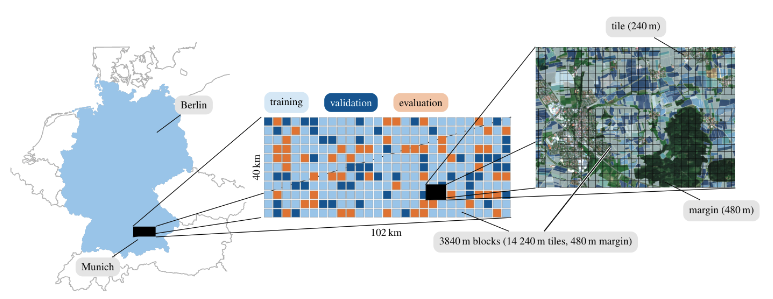
\includegraphics[width=\textwidth]{images/aoi}
\end{frame}



\begin{frame}[t]
\frametitle{Looking at Sequence to Sequence Models from NLP}
%	\framesubtitle{Natürlicher Sprachverarbeitung, Übersetzung, Spracherkennung}

%Verbreitet in sequenziellen Aufgabengebieten, wie natürlicher Sprachverarbeitung, Übersetzung, Spracherkennung
%	\begin{center}
%		\large Wort-Sequenz $\rightarrow$ Representation $c$ $\rightarrow$ Wort-Sequenz
%	\end{center}
\begin{center}
	%\tikzsetnextfilename{seq2seq}

\tikzstyle{operator} = [draw, circle, fill=tumbluemedium, draw=tumbluemedium, inner sep=0, text=white]
%\tikzstyle{function} = [draw, rectangle, fill=tumbluemedium, draw=tumbluemedium, text=white]
\tikzstyle{gate} = [fill=tumivory,draw,rounded corners]

\tikzstyle{dummy} = [inner sep=0]
\tikzstyle{flow} = [rounded corners]
\tikzstyle{endflow} = [-stealth,flow]
\tikzstyle{beginflow} = [stealth-,flow]

\tikzstyle{bigbox} = [rectangle, draw=tumivory, thick, fill=tumgraylight, rounded corners, 
inner sep=.5ex]

\tikzstyle{bigpassbox} = [opacity=.2, rounded corners, draw=none]


\tikzset{pic shift/.store in=\shiftcoord,
	pic shift={(0,0)},
	pics/seqlstmencoder/.style={
		code={
		\begin{scope}[shift={\shiftcoord},xscale=1.3,yscale=.9]
			
			\node[dummy] (bl) at (0,0){}; % bottom left
			\node[dummy] (tr) at (1,1){}; % top right
			
			\node[dummy] (br) at ($ (bl -| tr) $){}; % bottom right
			\node[dummy] (tl) at ($ (bl |- tr) $){}; % top left
			
			\node[fit=(bl) (tr),bigbox] (-C) {};
			
			% input coordinate for rounded draw lines -> slightly right of tl
			\coordinate (-input) at (0.1,1); % top left
			
			% output coordinate for rounded draw lines -> slightly left of br
			\coordinate (-coutput) at (0.9,0); % bottom right
			\coordinate (-cinput) at (0.1,0); % bottom left
			\coordinate (-houtput) at (0.9,1); % bottom right
			
%			% gate distance
			\def\d{1/6}
			
			% gate heights
			\def\h{1/3}
			
			\coordinate (f)  at bl+(1*\d,0);
			\coordinate (i)  at bl+(2*\d,0);
			\coordinate (j)  at bl+(3*\d,0);
			\coordinate (o)  at bl+(4*\d,0);
			\coordinate (out) at bl+(5*\d,0);
			
			\coordinate (gates) at (0,2*\h);
			
			%\node[above=of tl](xt){$x_{t}$};
			%\node[left=of tl](htminus1){$h_{t-1}$};
			
			%\node[below=of br](ct){$c_{t}$};
			
			\node[gate](fgate) at ($ (gates -| f) $){};
			\node[gate](igate) at ($ (gates -| i) $){};
			\node[gate](jgate) at ($ (gates -| j) $){};
			\node[gate](ogate) at ($ (gates -| o) $){};
			
%			\coordinate (htminus1) at bl+(-.5,0);
%			\coordinate (ht) at bl+(-.5,0);
%			
			% forget gate
			\node[operator](fmult) at ($ (bl -| fgate) $) {};
			\draw[endflow] (-input) -| (fgate) -- (fmult); 
			
%			%j
			\node[operator](jmult) at ([shift={(0,-1*\h)}]jgate) {};
			\node[operator](cadd) at ($ (bl -| jgate) $) {};
			\draw[endflow] (-input) -| (jgate) -- (jmult);
			\draw[endflow] (jmult) -- (cadd); 			

%			%i	
			\draw[endflow] (-input) -| (igate) |- (jmult); 
%
%%			% outpu
			\node[operator](outtanh) at ([shift={(0,1*\h)}]out) {};
%			
%			%o 
			\draw[endflow] (tl) -| (ogate) |- (outtanh);
			\draw[flow] (outtanh) |- (-houtput);
%			
%			% output flow
			\draw[endflow] (cadd) -| (outtanh);
			\draw[flow] (-cinput) -- (fmult) -- (cadd) -- (-coutput);
%			
			
			% debug
%			\node at (gates) {\tiny{gates}};
%			\node at (-input) {\tiny{-input}};
%			\node at (-coutput) {\tiny{-coutput}};
%			\node at (-houtput) {\tiny{-houtput}};
%			\node at (f) {\tiny{f}};
%			\node at (i) {\tiny{i}};
%			\node at (j) {\tiny{j}};
%			\node at (o) {\tiny{o}};
%			\node at (tl) {\tiny{tl}};
%			\node at (br) {\tiny{br}};
%			\node at (bl) {\tiny{bl}};
%			\node at (tr) {\tiny{tr}};
%			\node at (out) {\tiny{out}};
			
		\end{scope}
		}
	}
}
\tikzset{pic shift/.store in=\shiftcoord,
	pic shift={(0,0)},
	pics/seqlstmdecoder/.style={
		code={
			\begin{scope}[shift={\shiftcoord},xscale=1.3,yscale=-.9]
				
				\node[dummy] (bl) at (0,0){}; % bottom left
				\node[dummy] (tr) at (1,1){}; % top right
				
				\node[dummy] (br) at ($ (bl -| tr) $){}; % bottom right
				\node[dummy] (tl) at ($ (bl |- tr) $){}; % top left
				
				\node[fit=(bl) (tr),bigbox] (-C) {};
				
				% input coordinate for rounded draw lines -> slightly right of tl
				\coordinate (-input) at (0.1,1); % top left
				
				% output coordinate for rounded draw lines -> slightly left of br
				\coordinate (-coutput) at (0.9,0); % bottom right
				\coordinate (-cinput) at (0.1,0); % bottom left
				\coordinate (-houtput) at (0.9,1); % top right
				
				%			% gate distance
				\def\d{1/6}
				
				% gate heights
				\def\h{1/3}
				
				\coordinate (f)  at bl+(1*\d,0);
				\coordinate (i)  at bl+(2*\d,0);
				\coordinate (j)  at bl+(3*\d,0);
				\coordinate (o)  at bl+(4*\d,0);
				\coordinate (out) at bl+(5*\d,0);
				
				\coordinate (gates) at (0,2*\h);
				
				%\node[above=of tl](xt){$x_{t}$};
				%\node[left=of tl](htminus1){$h_{t-1}$};
				
				%\node[below=of br](ct){$c_{t}$};
				
				\node[gate](fgate) at ($ (gates -| f) $){};
				\node[gate](igate) at ($ (gates -| i) $){};
				\node[gate](jgate) at ($ (gates -| j) $){};
				\node[gate](ogate) at ($ (gates -| o) $){};
				
				%			\coordinate (htminus1) at bl+(-.5,0);
				%			\coordinate (ht) at bl+(-.5,0);
				%			
				% forget gate
				\node[operator](fmult) at ($ (bl -| fgate) $) {};
				\draw[endflow] (-input) -| (fgate) -- (fmult); 
				
				%			%j
				\node[operator](jmult) at ([shift={(0,-1*\h)}]jgate) {};
				\node[operator](cadd) at ($ (bl -| jgate) $) {};
				\draw[endflow] (-input) -| (jgate) -- (jmult);
				\draw[endflow] (jmult) -- (cadd); 			
				
				%			%i	
				\draw[endflow] (-input) -| (igate) |- (jmult); 
				%
				%%			% outpu
				\node[operator](outtanh) at ([shift={(0,1*\h)}]out) {};
				%			
				%			%o 
				\draw[endflow] (tl) -| (ogate) |- (outtanh);
				\draw[flow] (outtanh) |- (-houtput);
				%			
				%			% output flow
				\draw[endflow] (cadd) -| (outtanh);
				\draw[flow] (-cinput) -- (fmult) -- (cadd) -- (-coutput);
				%			
				
				% debug
				%			\node at (gates) {\tiny{gates}};
				%			\node at (-input) {\tiny{-input}};
				%			\node at (-coutput) {\tiny{-coutput}};
				%			\node at (-houtput) {\tiny{-houtput}};
				%			\node at (f) {\tiny{f}};
				%			\node at (i) {\tiny{i}};
				%			\node at (j) {\tiny{j}};
				%			\node at (o) {\tiny{o}};
				%			\node at (tl) {\tiny{tl}};
				%			\node at (br) {\tiny{br}};
				%			\node at (bl) {\tiny{bl}};
				%			\node at (tr) {\tiny{tr}};
				%			\node at (out) {\tiny{out}};
				
			\end{scope}
		}
	}
}


\begin{tikzpicture}[scale=1, node distance=2em]%,show background rectangle,background rectangle/.style={draw=red}]

%\matrix (m) [matrix of nodes, ampersand replacement=\&]{

\def\d{1.8}
\def\encoderheight{0}
\def\decoderheight{-1.3}

\draw pic (enc1) at (\d,\encoderheight) {seqlstmencoder};% \&
\node[above=of enc1tl](xenc1){I};

\draw pic (enc2) at (2*\d,\encoderheight) {seqlstmencoder};
\node[above=of enc2-input](xenc2){live};

\draw pic (enc3) at (3*\d,\encoderheight) {seqlstmencoder};
\node[above=of enc3-input](xenc3){in};

\draw pic (enc4) at (4*\d,\encoderheight) {seqlstmencoder};
\node[above=of enc4-input](xenc4){Munich};

\draw pic (dec1) at (1*\d,\decoderheight) {seqlstmdecoder};% \&
\node[below=of dec1tr](ydec1){Ich};

\draw pic (dec2) at (2*\d,\decoderheight) {seqlstmdecoder};
\node[below=of dec2tr](ydec2){lebe};

\draw pic (dec3) at (3*\d,\decoderheight) {seqlstmdecoder};
\node[below=of dec3tr](ydec3){in};

\draw pic (dec4) at (4*\d,\decoderheight) {seqlstmdecoder};
\node[below=of dec4tr](ydec4){München};

\node[anchor=center](state) at ($(enc4-coutput)!0.5!(dec1-cinput)$){representation $\VCellState_T$};

\node[left=of enc1-input](enczerostateh){$\V{0}$};
\node[left=of enc1-cinput](enczerostatec){$\V{0}$};
\node[left=of dec1-input](deczerostateh){$\V{0}$};

\draw[endflow] (enczerostateh) -- (enc1-input);
\draw[endflow] (enczerostatec) -- (enc1-cinput);
\draw[endflow] (deczerostateh) -- (dec1-input);


% draw state
\draw[flow] (enc4-coutput) -- ++(.2,0) |- (state);
\draw[beginflow] (dec1-cinput) -- ++(-.2,0) |- (state);

% draw connections from input to cells
\draw[flow] (xenc1) |- (enc1-input);
\draw[flow] (xenc2) |- (enc2-input);
\draw[flow] (xenc3) |- (enc3-input);
\draw[flow] (xenc4) |- (enc4-input);

% draw connections from cells to output
\draw[beginflow] (ydec1) |- (dec1-houtput);
\draw[beginflow] (ydec2) |- (dec2-houtput);
\draw[beginflow] (ydec3) |- (dec3-houtput);
\draw[flow] (ydec4) |- (dec4-houtput);

% draw hidden connections between cells
\draw[endflow] (enc1-houtput) -- (enc2-input);
\draw[endflow] (enc2-houtput) -- (enc3-input);
\draw[endflow] (enc3-houtput) -- (enc4-input);

\draw[endflow] (dec1-houtput) -- (dec2-input);
\draw[endflow] (dec2-houtput) -- (dec3-input);
\draw[endflow] (dec3-houtput) -- (dec4-input);

% draw hidden connections between cells
\draw[endflow] (enc1-coutput) -- (enc2-cinput);
\draw[endflow] (enc2-coutput) -- (enc3-cinput);
\draw[endflow] (enc3-coutput) -- (enc4-cinput);

\draw[endflow] (dec1-coutput) -- (dec2-cinput);
\draw[endflow] (dec2-coutput) -- (dec3-cinput);
\draw[endflow] (dec3-coutput) -- (dec4-cinput);

%\node[bigpassbox, fill=classcolor, rectangle, minimum width=4cm,minimum height=3.5cm, anchor=center, label={[shift={(-1ex,-3.5ex)}]north:classification}] (classbox) at (13,0) {};
%};

\end{tikzpicture}
\end{center}
%\begin{columns}
%	\column{.4\textwidth}
%	%		\brand{Word2Vec} embedding 
%	%		Neural Machine Translation encodes 
%	
%	\centering 
%%	
%%	\begin{tikzpicture}
%%	\node[fill=tumbluelight!50,rounded corners](x){Eingabesequenz};
%%	\node[fill=tumbluelight!50,rounded corners, below=of x](c){Repräsentation};
%%	\node[fill=tumbluelight!50,rounded corners, below=of c](o){Ausgabsequenz};
%%	
%%	\draw[-stealth] (x) -- (c);
%%	\draw[-stealth] (c) -- (o);
%%	
%%	\end{tikzpicture}
%%	
%	\column{.6\textwidth}
%	
%\end{columns}


{\small
	Sutskever, I., Vinyals, O., \& Le, Q. V. (2014). Sequence to sequence learning with neural networks. In Advances in neural information processing systems (pp. 3104-3112).}


\end{frame}

%\tikzsetnextfilename{network}

\tikzstyle{operator} = [draw, circle, fill=tumbluemedium, draw=tumbluemedium, inner sep=0, text=white]
%\tikzstyle{function} = [draw, rectangle, fill=tumbluemedium, draw=tumbluemedium, text=white]
\tikzstyle{gate} = [fill=tumivory,draw,rounded corners]

\tikzstyle{dummy} = [inner sep=0]
\tikzstyle{flow} = [rounded corners]
\tikzstyle{endflow} = [-stealth,flow]
\tikzstyle{beginflow} = [stealth-,flow]

\tikzstyle{bigpassbox} = [opacity=.2, rounded corners, draw=none]

% defaultvalue -> might be replaced later
\colorlet{tensorcolor}{tumblue}

\tikzstyle{bigbox} = [rectangle, draw=tumivory, thick, fill=tumgraylight, rounded corners, 
inner sep=.5ex]

\tikzstyle{wireframe} = [draw=tumgray]
\tikzstyle{image} = [inner sep=0, fill=none, minimum size=\imagewidth]

\tikzset{pic shift/.store in=\shiftcoord,
	pic shift={(0,0)},
	pics/seqlstmfw/.style={
		code={
		\begin{scope}[shift={\shiftcoord},xscale=1.3,yscale=.8]
			
			\node[dummy] (bl) at (0,0){}; % bottom left
			\node[dummy] (tr) at (1,1){}; % top right
			
			\node[dummy] (br) at ($ (bl -| tr) $){}; % bottom right
			\node[dummy] (tl) at ($ (bl |- tr) $){}; % top left
			
			\node[fit=(bl) (tr),bigbox] (-C) {};
			
			% input coordinate for rounded draw lines -> slightly right of tl
			\coordinate (-input) at (0.1,1); % top left
			
			% output coordinate for rounded draw lines -> slightly left of br
			\coordinate (-coutput) at (0.9,0); % bottom right
			\coordinate (-cinput) at (0.1,0); % bottom left
			\coordinate (-houtput) at (0.9,1); % bottom right
			
%			% gate distance
			\def\d{1/6}
			
			% gate heights
			\def\h{1/3}
			
			\coordinate (f)  at bl+(1*\d,0);
			\coordinate (i)  at bl+(2*\d,0);
			\coordinate (j)  at bl+(3*\d,0);
			\coordinate (o)  at bl+(4*\d,0);
			\coordinate (out) at bl+(5*\d,0);
			
			\coordinate (gates) at (0,2*\h);
			
			%\node[above=of tl](xt){$x_{t}$};
			%\node[left=of tl](htminus1){$h_{t-1}$};
			
			%\node[below=of br](ct){$c_{t}$};
			
			\node[gate](fgate) at ($ (gates -| f) $){};
			\node[gate](igate) at ($ (gates -| i) $){};
			\node[gate](jgate) at ($ (gates -| j) $){};
			\node[gate](ogate) at ($ (gates -| o) $){};
			
%			\coordinate (htminus1) at bl+(-.5,0);
%			\coordinate (ht) at bl+(-.5,0);
%			
			% forget gate
			\node[operator](fmult) at ($ (bl -| fgate) $) {};
			\draw[endflow] (-input) -| (fgate) -- (fmult); 
			
%			%j
			\node[operator](jmult) at ([shift={(0,-1*\h)}]jgate) {};
			\node[operator](cadd) at ($ (bl -| jgate) $) {};
			\draw[endflow] (-input) -| (jgate) -- (jmult);
			\draw[endflow] (jmult) -- (cadd); 			

%			%i	
			\draw[endflow] (-input) -| (igate) |- (jmult); 
%
%%			% outpu
			\node[operator](outtanh) at ([shift={(0,1*\h)}]out) {};
%			
%			%o 
			\draw[endflow] (tl) -| (ogate) |- (outtanh);
			\draw[flow] (outtanh) |- (-houtput);
%			
%			% output flow
			\draw[endflow] (cadd) -| (outtanh);
			\draw[flow] (-cinput) -- (fmult) -- (cadd) -- (-coutput);
%			
			
			% debug
%			\node at (gates) {\tiny{gates}};
%			\node at (-input) {\tiny{-input}};
%			\node at (-coutput) {\tiny{-coutput}};
%			\node at (-houtput) {\tiny{-houtput}};
%			\node at (f) {\tiny{f}};
%			\node at (i) {\tiny{i}};
%			\node at (j) {\tiny{j}};
%			\node at (o) {\tiny{o}};
%			\node at (tl) {\tiny{tl}};
%			\node at (br) {\tiny{br}};
%			\node at (bl) {\tiny{bl}};
%			\node at (tr) {\tiny{tr}};
%			\node at (out) {\tiny{out}};
			
		\end{scope}
		}
	}
}

\tikzset{pic shift/.store in=\shiftcoord,
	pic shift={(0,0)},
	pics/seqlstmbw/.style={
		code={
			\begin{scope}[shift={\shiftcoord},xscale=1.3,yscale=-.8]
				
				\node[dummy] (bl) at (0,0){}; % bottom left
				\node[dummy] (tr) at (1,1){}; % top right
				
				\node[dummy] (br) at ($ (bl -| tr) $){}; % bottom right
				\node[dummy] (tl) at ($ (bl |- tr) $){}; % top left
				
				\node[fit=(bl) (tr),bigbox] (-C) {};
				
				% input coordinate for rounded draw lines -> slightly right of tl
				\coordinate (-input) at (0.1,1); % top left
				
				% output coordinate for rounded draw lines -> slightly left of br
				\coordinate (-coutput) at (0.9,0); % bottom right
				\coordinate (-cinput) at (0.1,0); % bottom left
				\coordinate (-houtput) at (0.9,1); % top right
				
				%			% gate distance
				\def\d{1/6}
				
				% gate heights
				\def\h{1/3}
				
				\coordinate (f)  at bl+(1*\d,0);
				\coordinate (i)  at bl+(2*\d,0);
				\coordinate (j)  at bl+(3*\d,0);
				\coordinate (o)  at bl+(4*\d,0);
				\coordinate (out) at bl+(5*\d,0);
				
				\coordinate (gates) at (0,2*\h);
				
				%\node[above=of tl](xt){$x_{t}$};
				%\node[left=of tl](htminus1){$h_{t-1}$};
				
				%\node[below=of br](ct){$c_{t}$};
				
				\node[gate](fgate) at ($ (gates -| f) $){};
				\node[gate](igate) at ($ (gates -| i) $){};
				\node[gate](jgate) at ($ (gates -| j) $){};
				\node[gate](ogate) at ($ (gates -| o) $){};
				
				%			\coordinate (htminus1) at bl+(-.5,0);
				%			\coordinate (ht) at bl+(-.5,0);
				%			
				% forget gate
				\node[operator](fmult) at ($ (bl -| fgate) $) {};
				\draw[endflow] (-input) -| (fgate) -- (fmult); 
				
				%			%j
				\node[operator](jmult) at ([shift={(0,-1*\h)}]jgate) {};
				\node[operator](cadd) at ($ (bl -| jgate) $) {};
				\draw[endflow] (-input) -| (jgate) -- (jmult);
				\draw[endflow] (jmult) -- (cadd); 			
				
				%			%i	
				\draw[endflow] (-input) -| (igate) |- (jmult); 
				%
				%%			% outpu
				\node[operator](outtanh) at ([shift={(0,1*\h)}]out) {};
				%			
				%			%o 
				\draw[endflow] (tl) -| (ogate) |- (outtanh);
				\draw[flow] (outtanh) |- (-houtput);
				%			
				%			% output flow
				\draw[endflow] (cadd) -| (outtanh);
				\draw[flow] (-cinput) -- (fmult) -- (cadd) -- (-coutput);
				%			
				
				% debug
				%			\node at (gates) {\tiny{gates}};
				%			\node at (-input) {\tiny{-input}};
				%			\node at (-coutput) {\tiny{-coutput}};
				%			\node at (-houtput) {\tiny{-houtput}};
				%			\node at (f) {\tiny{f}};
				%			\node at (i) {\tiny{i}};
				%			\node at (j) {\tiny{j}};
				%			\node at (o) {\tiny{o}};
				%			\node at (tl) {\tiny{tl}};
				%			\node at (br) {\tiny{br}};
				%			\node at (bl) {\tiny{bl}};
				%			\node at (tr) {\tiny{tr}};
				%			\node at (out) {\tiny{out}};
				
			\end{scope}
		}
	}
}

%\newcommand{}{
%	\begin{tikzpicture}
%	% each layer
%	\begin{scope}[scale=2]
%	
%	% raster size
%	\def\d{0.7}		
%	
%	% distance layer
%	\def\s{\d*5}
%	
%	\foreach \i in {1,...,6}
%	{		
%		\begin{scope}[
%		yshift=\s*\i,every node/.append style={
%			yslant=0.5,xslant=-1},yslant=0.5,xslant=-1
%		]
%		%\draw[step=3.33mm] (0,0) grid (1,1);
%		%\fill[black,fill opacity=.9] (0.333,0.333) rectangle (0.333,0.333);    	    	  
%		
%		\foreach \row in {0,...,2}{
%			\foreach \col in {0,...,2}{
%				\draw[tumblack, fill=tumblue!\pdfuniformdeviate 40,fill opacity=1,rounded corners=1] (\col*\d/3,\row*\d/3) rectangle (\col*\d/3+\d/3, \row*\d/3+\d/3);
%				%                 \draw[black, fill=black!\pdfuniformdeviate 40,fill opacity=1,rounded corners=1] (\col*\d/3,\row*\d/3) rectangle (\col*\d/3+\d/3, \row*\d/3+\d/3);
%			}
%		}
%		
%		%\draw[step=3.33mm] (0,0) grid (1,1);
%		%\fill[white,fill opacity=.9] (0,0) rectangle (1,1);
%		\end{scope}
%	}
%	\end{scope}
%	\end{tikzpicture}
%}
%%
%\newcommand{}{
%	
%	\begin{tikzpicture}[scale=2]
%	\foreach \i in {0,...,9}
%	\draw[tumblack,fill=tumorange!\pdfuniformdeviate 40,fill opacity=.9, rounded corners=0.5] (\i*.2, 0) rectangle (\i*.2+.2, .2);
%	\end{tikzpicture}
%}

\newcommand{\figencoderfieldRNN}{
	
	\begin{tikzpicture}[scale=1, node distance=1em]%,show background rectangle,background rectangle/.style={draw=red}]
	
	%\matrix (m) [matrix of nodes, ampersand replacement=\&]{
	
	\def\d{1.7}
	\def\encoderheight{0.4}
	\def\decoderheight{-0.4}
	\def\imagewidth{8mm}
	\def\stateimagewidth{8mm}
	\def\classimagewidth{8mm}
	
	\def\rgbone{images/network/48px/rgb1}
	\def\rgbtwo{images/network/48px/rgb2}
	\def\rgbthree{images/network/48px/rgb3}
	\def\rgbfour{images/network/48px/rgb4}
	\def\prediction{images/network/48px/prediction}
	\def\groundtruth{images/network/48px/ground_truth}
	\def\activation{images/network/48px/maize}
	\def\state{images/network/48px/state}
	
	
	%\draw [bigpassbox, fill=forwardcolor](1,.25) rectangle (10,4);
	
	\node[bigpassbox, fill=none, rectangle, minimum width=7cm,minimum height=3cm, anchor=south west, label={[shift={(2em,-3.5ex)}]north:}] (forwardbox) at (1,.15) {};
	%\draw [bigpassbox, fill=backwardcolor](1,-.25) rectangle (10,-4);
	
	\draw pic (fw1) at (\d,\encoderheight) {seqlstmfw};% \&
	\node[above=of fw1tl, label=above:{$\VInput_{1}$}](xfw1){
		
	};%images/network/time1_x
	
	\node[below= 3.5emof fw1-houtput, xshift=.5em, label=below:{$\V{y}_{1}$}](yfw1){
		
	};%images/network/time1_x
	
	\draw pic (fw2) at (2*\d,\encoderheight) {seqlstmfw};
	\node[above=of fw2-input, label=above:{$\VInput_{2}$}](xfw2){
		
	}; % images/network/time11_x
	
	\node[below= 3.5emof fw2-houtput, xshift=.5em, label=below:{$\V{y}_{2}$}](yfw2){
		
	};%images/network/time1_x
	
	\draw pic (fw3) at (3*\d,\encoderheight) {seqlstmfw};
	\node[above=of fw3-input](xfw3){$\dots$};
	\node[below= 3.5emof fw3-houtput, xshift=.5em](yfw3){
		%	
		$\dots$
	};%images/network/time1_x
	
	\draw pic (fw4) at (4*\d,\encoderheight) {seqlstmfw};
	\node[above=of fw4-input, label=above:{$\VInput_T$}](xfw4){
		
	}; % images/network/time30_x
	
	\node[below= 3.5emof fw4-houtput, xshift=.5em, label=below:{$\V{y}_{T}$}](yfw4){
		
	};%images/network/time1_x
	
	\node[left=of fw1-input](enczerostateh){$\V{0}$};
	\node[left=of fw1-cinput](enczerostatec){$\V{0}$};
	\draw[endflow] (enczerostateh) -- (fw1-input);
	\draw[endflow] (enczerostatec) -- (fw1-cinput);
	
	% draw connections from input to cells
	\draw[flow] (xfw1) |- (fw1-input);
	\draw[flow] (xfw2) |- (fw2-input);
	\draw[flow] (xfw3) |- (fw3-input);
	\draw[flow] (xfw4) |- (fw4-input);
	
	% draw hidden connections between cells
	\draw[endflow] (fw1-houtput) -- (fw2-input);
	\draw[endflow] (fw2-houtput) -- (fw3-input);
	\draw[endflow] (fw3-houtput) -- (fw4-input);
	
	% draw hidden connections between cells
	\draw[endflow] (fw1-coutput) -- (fw2-cinput);
	\draw[endflow] (fw2-coutput) -- (fw3-cinput);
	\draw[endflow] (fw3-coutput) -- (fw4-cinput);
	
	% outputs
	\draw[endflow] (fw1-houtput) -- ($ (fw1-houtput)+(.5em,0) $) -- (yfw1);
	\draw[endflow] (fw2-houtput) -- ($ (fw2-houtput)+(.5em,0) $) -- (yfw2);
	\draw[endflow] (fw3-houtput) -- ($ (fw3-houtput)+(.5em,0) $) -- (yfw3);
	\draw[endflow] (fw4-houtput) -- ($ (fw4-houtput)+(.5em,0) $) -- (yfw4);
	
	%\node[right= 2.5em of fw4-coutput](cfw){$\VCellState_T^\text{fw}$};
	
	%\draw[endflow] (fw4-coutput) -- (cfw);
	
	%};
	\end{tikzpicture}
}

\newcommand{\figencoder}{

\begin{tikzpicture}[scale=1, node distance=1em]%,show background rectangle,background rectangle/.style={draw=red}]

%\matrix (m) [matrix of nodes, ampersand replacement=\&]{

\def\d{1.7}
\def\encoderheight{0.4}
\def\decoderheight{-0.4}
\def\imagewidth{8mm}
\def\stateimagewidth{8mm}
\def\classimagewidth{8mm}

\def\rgbone{images/network/48px/rgb1}
\def\rgbtwo{images/network/48px/rgb2}
\def\rgbthree{images/network/48px/rgb3}
\def\rgbfour{images/network/48px/rgb4}
\def\prediction{images/network/48px/prediction}
\def\groundtruth{images/network/48px/ground_truth}
\def\activation{images/network/48px/maize}
\def\state{images/network/48px/state}


%\draw [bigpassbox, fill=forwardcolor](1,.25) rectangle (10,4);

\node[bigpassbox, fill=none, rectangle, minimum width=7cm,minimum height=3cm, anchor=south west, label={[shift={(2em,-3.5ex)}]north:}] (forwardbox) at (1,.15) {};
%\draw [bigpassbox, fill=backwardcolor](1,-.25) rectangle (10,-4);

\draw pic (fw1) at (\d,\encoderheight) {seqlstmfw};% \&
\node[above=of fw1tl, label=above:{$\VInput_{1}$}](xfw1){\includegraphics[width=\imagewidth]{\rgbone}};%images/network/time1_x

\draw pic (fw2) at (2*\d,\encoderheight) {seqlstmfw};
\node[above=of fw2-input, label=above:{$\VInput_{2}$}](xfw2){\includegraphics[width=\imagewidth]{\rgbtwo}}; % images/network/time11_x

\draw pic (fw3) at (3*\d,\encoderheight) {seqlstmfw};
\node[above=of fw3-input](xfw3){$\dots$};

\draw pic (fw4) at (4*\d,\encoderheight) {seqlstmfw};
\node[above=of fw4-input, label=above:{$\VInput_T$}](xfw4){\includegraphics[width=\imagewidth]{\rgbfour}}; % images/network/time30_x

\node[left=of fw1-input](enczerostateh){$\V{0}$};
\node[left=of fw1-cinput](enczerostatec){$\V{0}$};
\draw[endflow] (enczerostateh) -- (fw1-input);
\draw[endflow] (enczerostatec) -- (fw1-cinput);

% draw connections from input to cells
\draw[flow] (xfw1) |- (fw1-input);
\draw[flow] (xfw2) |- (fw2-input);
\draw[flow] (xfw3) |- (fw3-input);
\draw[flow] (xfw4) |- (fw4-input);

% draw hidden connections between cells
\draw[endflow] (fw1-houtput) -- (fw2-input);
\draw[endflow] (fw2-houtput) -- (fw3-input);
\draw[endflow] (fw3-houtput) -- (fw4-input);

% draw hidden connections between cells
\draw[endflow] (fw1-coutput) -- (fw2-cinput);
\draw[endflow] (fw2-coutput) -- (fw3-cinput);
\draw[endflow] (fw3-coutput) -- (fw4-cinput);

\node[right= 2.5em of fw4-coutput](cfw){$\VCellState_T^\text{fw}$};

\draw[endflow] (fw4-coutput) -- (cfw);

%};
\end{tikzpicture}

}
\begin{frame}
\frametitle{Temporal Vegetation Modelling with LSTMs}
\framesubtitle{CVPR Earthvision 2017}
\begin{columns}
	\column{.5\textwidth}
	\figencoderfieldRNN
	\column{.5\textwidth}
	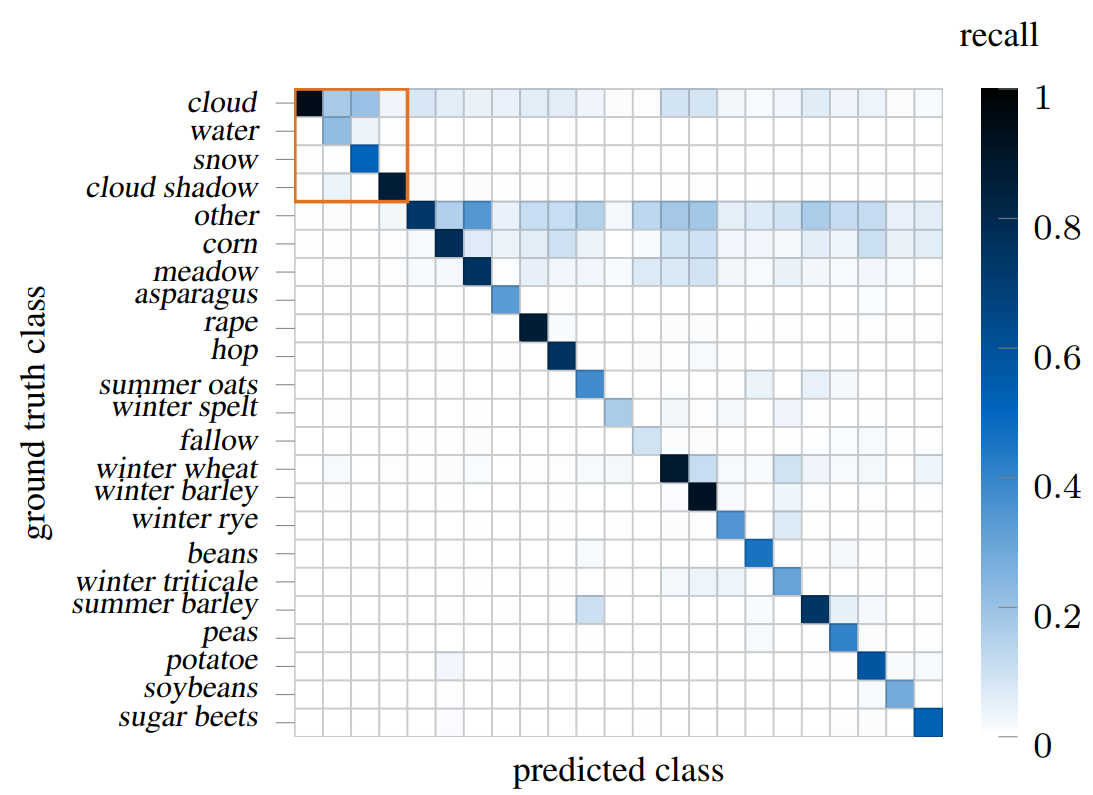
\includegraphics[width=.8\textwidth]{images/confmat_fieldrnn}
%		images/stmelfadditional/Genauigkeiten/accuracies1}
\end{columns}

\vspace{1em}

\textsl{\small
	Rußwurm, M. and Körner, M. (2017). \textbf{Temporal Vegetation Modelling using Long Short-Term Memory Networks for Crop Identification from Medium-Resolution Multi-Spectral Satellite Images}. In IEEE/ISPRS EarthVision 2017 Workshop, Proceedings of the IEEE CVPR Workshops. \textbf{\color{tumorange} Best Paper Award}
}

\end{frame}



\def\fps{3}
%\tikzsetnextfilename{lstm}

\tikzstyle{operator} = [draw, circle, fill=tumbluemedium, draw=tumbluemedium, inner sep=0, text=white]
%\tikzstyle{function} = [draw, rectangle, fill=tumbluemedium, draw=tumbluemedium, text=white]
\tikzstyle{gate} = [fill=tumivory,draw,rounded corners=1pt, inner sep=2pt, minimum width=11mm, minimum height=11mm]
\tikzstyle{io} = [fill=tumwhite,draw,rounded corners=1pt, inner sep=2pt, minimum width=11mm, minimum height=11mm]

\tikzstyle{dummy} = [inner sep=0]
\tikzstyle{flow} = [rounded corners]
\tikzstyle{endflow} = [-stealth,flow]

\colorlet{boxcolor}{tumgraylight}
\tikzstyle{bigbox} = [rectangle, draw=tumivory, thick, fill=boxcolor, rounded corners, 
inner xsep=0ex, inner ysep=2ex]

\tikzset{pic shift/.store in=\shiftcoord,
	pic shift={(0,0)},
	lstmexplain/.pic = {
		\begin{scope}[shift={\shiftcoord},xscale=6,yscale=2.5]
			
			\node[dummy] (bl) at (0,0){}; % bottom left
			\node[dummy] (tr) at (1,1){}; % top right
			
			\node[dummy] (br) at ($ (bl -| tr) $){}; % bottom right
			\node[dummy] (tl) at ($ (bl |- tr) $){}; % top left
			
			\node[fit=(bl) (tr),bigbox] (-C) {};
			
			% input coordinate for rounded draw lines -> slightly right of tl
			\coordinate (-input) at (0.1,1); % top left
			
			% output coordinate for rounded draw lines -> slightly left of br
			\coordinate (-coutput) at (0.98,0); % bottom right
			\coordinate (-houtput) at (0.98,1); % bottom right
			
%			% gate distance
			\def\d{1/5}
			
			% gate heights
			\def\h{1/3}
			
			\coordinate (f)  at bl+(0.7*\d,0);
			\coordinate (i)  at bl+(1.8*\d,0);
			\coordinate (j)  at bl+(2.9*\d,0);
			\coordinate (o)  at bl+(4*\d,0);
			\coordinate (out) at bl+(4.7*\d,0);
			
			\coordinate (gates) at (0,2*\h);
			
			%\node[above=of tl](xt){$x_{t}$};
			%\node[left=of tl](htminus1){$h_{t-1}$};
			
			%\node[below=of br](ct){$c_{t}$};
%			\setlength{\thinmuskip}{0pt}
			
			\visible<2->{
			\node[gate](fgate) at ($ (gates -| f) $){
				$\VForgetGate_t$
				};
				\draw[endflow] (-input) -| (fgate);
			}
			
			\visible<3->{
			\node[gate](igate) at ($ (gates -| i) $){
				$\VInputGate_t$
				};
			}
				
			\visible<3->{
			\node[gate](jgate) at ($ (gates -| j) $){$\VModulationGate_t$};
			\node[operator](jmult) at ([shift={(0,-1.3*\h)}]jgate) {$ \odot $};
			\draw[endflow] (-input) -| (jgate);
			\draw[endflow] (jgate) -- (jmult);
			\draw[endflow] (-input) -| (igate); 
			\draw[endflow] (igate) |- (jmult);
			}
				
			\visible<4->{
			\node[gate](ogate) at ($ (gates -| o) $){
				$\VOutputGate_t$
				};
			\draw[endflow] (tl) -| (ogate);
			}
			
%			\coordinate (htminus1) at bl+(-.5,0);
%			\coordinate (ht) at bl+(-.5,0);
%			
			% forget gate 
			\visible<5->{
			\node[operator](fmult) at ($ (bl -| fgate) $) {$ \odot $};
			\draw[endflow] (fgate) -- (fmult); 
			\node[operator](cadd) at ($ (bl -| jgate) $) {$ + $};
			\draw[endflow] (jmult) -- (cadd); 
			\draw[flow] (fmult) -- (cadd) -- (-coutput);		
			}

			\visible<6->{
			\node[operator](outtanh) at ($ (jmult -| out) $) {$\odot$};
			\draw[endflow] (ogate) |- (outtanh);
			\draw[flow] (outtanh) |- (-houtput);
			\draw[endflow] (cadd) -| (outtanh);
			}
		\end{scope}
	}
}

\tikzset{pic shift/.store in=\shiftcoord,
	pic shift={(0,0)},
	lstmanim/.pic = {
		\begin{scope}[shift={\shiftcoord},xscale=6,yscale=2.5]
			
			\node[dummy] (bl) at (0,0){}; % bottom left
			\node[dummy] (tr) at (1,1){}; % top right
			
			\node[dummy] (br) at ($ (bl -| tr) $){}; % bottom right
			\node[dummy] (tl) at ($ (bl |- tr) $){}; % top left
			
			\node[fit=(bl) (tr),bigbox] (-C) {};
			
			% input coordinate for rounded draw lines -> slightly right of tl
			\coordinate (-input) at (0.1,1); % top left
			
			% output coordinate for rounded draw lines -> slightly left of br
			\coordinate (-coutput) at (0.98,0); % bottom right
			\coordinate (-houtput) at (0.98,1); % bottom right
			
			%			% gate distance
			\def\d{1/5}
			
			% gate heights
			\def\h{1/3}
			
			\coordinate (f)  at bl+(0.7*\d,0);
			\coordinate (i)  at bl+(1.8*\d,0);
			\coordinate (j)  at bl+(2.9*\d,0);
			\coordinate (o)  at bl+(4*\d,0);
			\coordinate (out) at bl+(4.7*\d,0);
			
			\coordinate (gates) at (0,2*\h);
			
			%\node[above=of tl](xt){$x_{t}$};
			%\node[left=of tl](htminus1){$h_{t-1}$};
			
			%\node[below=of br](ct){$c_{t}$};
			
			\node[gate, label={[label distance=0ex]265:$\VForgetGate_{t}$}](fgate) at ($ (gates -| f) $){
				\animategraphics[poster=25,width=1cm,autoplay,loop]{\fps}{images/activations/16494/f/3-}{1}{36}
				};
			\node[gate, label={[label distance=0ex]265:$\VInputGate_{t}$}](igate) at ($ (gates -| i) $){
				\animategraphics[poster=25,width=1cm,autoplay,loop]{\fps}{images/activations/16494/i/3-}{1}{36}
				};
			\node[gate, label={[label distance=0ex]265:$\VModulationGate_{t}$}](jgate) at ($ (gates -| j) $){
				\animategraphics[poster=25,width=1cm,autoplay,loop]{\fps}{images/activations/16494/j/3-}{1}{36}
				};
			\node[gate, label={[label distance=0ex]265:$\VOutputGate_{t}$}](ogate) at ($ (gates -| o) $){
				\animategraphics[poster=25,width=1cm,autoplay,loop]{\fps}{images/activations/16494/o/3-}{1}{36}
				};
			
			%			\coordinate (htminus1) at bl+(-.5,0);
			%			\coordinate (ht) at bl+(-.5,0);
			%			
			% forget gate
			\node[operator](fmult) at ($ (bl -| fgate) $) {$ \odot $};
			\draw[endflow] (-input) -| (fgate);
			\draw[endflow] (fgate) -- (fmult); 
			
			%			%j
			\node[operator](jmult) at ([shift={(0,-1.3*\h)}]jgate) {$ \odot $};
			\node[operator](cadd) at ($ (bl -| jgate) $) {$ + $};
			\draw[endflow] (-input) -| (jgate);
			\draw[endflow] (jgate) -- (jmult);
			\draw[endflow] (jmult) -- (cadd); 			
			
			%			%i	
			\draw[endflow] (-input) -| (igate);
			\draw[endflow] (igate) |- (jmult); 
			%
			%%			% outpu
			\node[operator](outtanh) at ($ (jmult -| out) $) {$\odot$};
			%			
			%			%o 
			\draw[endflow] (tl) -| (ogate);
			\draw[endflow] (ogate) |- (outtanh);
			\draw[flow] (outtanh) |- (-houtput);
			%			
			%			% output flow
			\draw[endflow] (cadd) -| (outtanh);
			\draw[flow] (fmult) -- (cadd) -- (-coutput);
			%			
			
		\end{scope}
	}
}

\tikzset{pic shift/.store in=\shiftcoord,
	pic shift={(0,0)},
	simplernn/.pic = {
		\begin{scope}[shift={\shiftcoord},xscale=2,yscale=.1]
			
			\node[dummy] (bl) at (0,0){}; % bottom left
			\node[dummy] (tr) at (1,1){}; % top right
			
			\node[dummy] (br) at ($ (bl -| tr) $){}; % bottom right
			\node[dummy] (tl) at ($ (bl |- tr) $){}; % top left
			
			\node[fit=(bl) (tr),bigbox] (-C) {};
			
			% input coordinate for rounded draw lines -> slightly right of tl
			\coordinate (-input) at (0.1,1); % top left
			
			% output coordinate for rounded draw lines -> slightly left of br
			\coordinate (-coutput) at (0.98,0); % bottom right
			\coordinate (-houtput) at (0.98,1); % bottom right
			
			%			% gate distance
			\def\d{1/5}
			
			% gate heights
			
			\node[] at ($ (-input)!0.5!(-houtput) $)(label){
				RNN
%				$\sigma(\concat{\VInput_t}{\VHidden_{t-1}}\MWeight$
			};
			\draw[endflow] (-input) -- (label);
			\draw[flow] (label) -- (-houtput);
			%\node[above=of tl](xt){$x_{t}$};
			%\node[left=of tl](htminus1){$h_{t-1}$};
			
			%\node[below=of br](ct){$c_{t}$};
			
%			\node[gate, label={[label distance=0ex]265:$\VForgetGate_{t}$}](fgate) at ($ (gates -| f) $){
%				\animategraphics[poster=25,width=1cm,autoplay,loop]{\fps}{images/activations/16494/f/3-}{1}{36}
%			};
%			\node[gate, label={[label distance=0ex]265:$\VInputGate_{t}$}](igate) at ($ (gates -| i) $){
%				\animategraphics[poster=25,width=1cm,autoplay,loop]{\fps}{images/activations/16494/i/3-}{1}{36}
%			};
%			\node[gate, label={[label distance=0ex]265:$\VModulationGate_{t}$}](jgate) at ($ (gates -| j) $){
%				\animategraphics[poster=25,width=1cm,autoplay,loop]{\fps}{images/activations/16494/j/3-}{1}{36}
%			};
%			\node[gate, label={[label distance=0ex]265:$\VOutputGate_{t}$}](ogate) at ($ (gates -| o) $){
%				\animategraphics[poster=25,width=1cm,autoplay,loop]{\fps}{images/activations/16494/o/3-}{1}{36}
%			};
			
			%			\coordinate (htminus1) at bl+(-.5,0);
			%			\coordinate (ht) at bl+(-.5,0);
			%			
			% forget gate
%			\node[operator](fmult) at ($ (bl -| fgate) $) {$ \odot $};
%			\draw[endflow] (-input) -| (fgate);
%			\draw[endflow] (fgate) -- (fmult); 
			
			%			%j
%			\node[operator](jmult) at ([shift={(0,-1.3*\h)}]jgate) {$ \odot $};
%			\node[operator](cadd) at ($ (bl -| jgate) $) {$ + $};
%			\draw[endflow] (-input) -| (jgate);
%			\draw[endflow] (jgate) -- (jmult);
%			\draw[endflow] (jmult) -- (cadd); 			
			
			%			%i	
%			\draw[endflow] (-input) -| (igate);
%			\draw[endflow] (igate) |- (jmult); 
			%
			%%			% outpu
%			\node[operator](outtanh) at ($ (jmult -| out) $) {$\odot$};
			%			
			%			%o 
%			\draw[endflow] (tl) -| (ogate);
%			\draw[endflow] (ogate) |- (outtanh);
%			\draw[flow] (outtanh) |- (-houtput);
			%			
			%			% output flow
%			\draw[endflow] (cadd) -| (outtanh);
%			\draw[flow] (fmult) -- (cadd) -- (-coutput);
			%			
			
		\end{scope}
	}
}

\tikzset{pic shift/.store in=\shiftcoord,
	pic shift={(0,0)},
	gru/.pic = {
		\begin{scope}[shift={\shiftcoord},xscale=6,yscale=2.5]
			
			\node[dummy] (bl) at (0,0){}; % bottom left
			\node[dummy] (tr) at (1,1){}; % top right
			
			\node[dummy] (br) at ($ (bl -| tr) $){}; % bottom right
			\node[dummy] (tl) at ($ (bl |- tr) $){}; % top left
			
			\node[fit=(bl) (tr),bigbox] (-C) {};
			
			%			% gate distance
			\def\d{1/5}
			
			% gate heights
			\def\h{1/4}
			
			
			% input coordinate for rounded draw lines -> slightly right of tl
			\coordinate (-xinput) at (0.3*\d,1); % top left
			\coordinate (-xinputflow) at (0.5*\d,1); % top left
			
			\coordinate (-hinput) at (0.2*\d,1); % top left
			\coordinate (-hinputflow) at (0.2*\d,.9); % top left
			
			% output coordinate for rounded draw lines -> slightly left of br
			\coordinate (-houtput) at (.98,1); % bottom right
			
			\coordinate (r)  at bl+(1*\d,0);
			\coordinate (rgap)at bl+(2*\d,0);
			\coordinate (u)  at bl+(3*\d,0);
			\coordinate (c)  at bl+(4*\d,0);
			
			\coordinate (out) at bl+(4.75*\d,0);
			
			\coordinate (abovegates) at (0,3.5*\h);
			\coordinate (gates) at (0,2.3*\h);
			\coordinate (belowgates) at ($(gates)!0.65!(bl)$);
			
			
%			\node[above=of tl](xt){$x_{t}$};
%			\node[left=of tl](htminus1){$h_{t-1}$};
			
			%\node[below=of br](ct){$c_{t}$};
			
			
			\node[gate](rgate) at ($ (gates -| r) $){r};
			\node[gate](ugate) at ($ (gates -| u) $){u};
			\node[gate](cgate) at ($ (gates -| c) $){$\tilde{\VHidden}$};
			
			\node[operator](cadd) at ($ (cgate |- bl) $) {$+$};
			\node[operator](cmult) at ($ (cgate |- belowgates) $) {$\odot$};
			
			\node[operator](rmult) at ($ (rgap |- belowgates) $) {$\odot$};
			
			\node[operator](umult) at ($ (u |- bl) $) {$\odot$};
			\draw[endflow] (ugate) -- (umult); 
			
			\draw[endflow] (-hinput)++(0,-.1) |- ($ (bl -| rgate) $) -| (rmult); 
			\draw[endflow] (rgate) |- (rmult);
			
			\draw[endflow] (cgate) -- (cmult);
			\draw[endflow] (ugate) |- (cmult);
			\draw[endflow] (cmult) -- (cadd);
			
			
			%%			
			\draw[endflow] (-xinputflow) -| (rgate); 
			\draw[endflow] (-xinputflow) -| ($ (rgate |- abovegates) $) -| (ugate); 
%%			\draw[endflow] (rgate) |- ++(.5\d,-\h) -| (rgate); 
			
			\draw[flow, draw=boxcolor,double=black,double distance=\pgflinewidth,ultra thick] (rmult) |- ($ (ugate |- tl) $);
			
			
			%\draw[flow] (tl) |- ($ (abovegates -| u) $) -| (ugate); 
			\draw[endflow] (-xinputflow) -| (cgate); 
			\draw[flow] (-hinput)++(-0.1, 0) -- (-xinputflow); 
			
			\draw[flow] (-hinputflow) |- (umult) -- (cadd) -| ($ (out) + (0,.5) $) |- (-houtput); %($(br)!0.5!(tr)$) 
			
			
			
			%% debug
%			\node at (gates) {\tiny{gates}};
%			\node at (abovegates) {\tiny{abovegates}};
%			\node at (belowgates) {\tiny{belowgates}};
%			\node at (-input) {\tiny{-input}};
%			\node at (-coutput) {\tiny{-coutput}};
%			\node at (-houtput) {\tiny{-houtput}};
%			\node at (f) {\tiny{f}};
%			\node at (i) {\tiny{i}};
%			\node at (j) {\tiny{j}};
%			\node at (o) {\tiny{o}};
%			\node at (tl) {\tiny{tl}};
%			\node at (br) {\tiny{br}};
%			\node at (bl) {\tiny{bl}};
%			\node at (tr) {\tiny{tr}};
%			\node at (out) {\tiny{out}};
			
		\end{scope}
	}
}

\tikzset{pic shift/.store in=\shiftcoord,
	pic shift={(0,0)},
	concat/.pic = {
		\node[](a) at (0, .5){$\V{a}$};
		\node[](b) at (0, -.5){$\V{b}$};
		\node[](out) at (1, 0){$\concat{ \V{a} }{ \V{b} }$};
		
		\draw[endflow] (a) |- (out);
		\draw[endflow] (b) |- (out);
	}
}

\tikzset{pic shift/.store in=\shiftcoord,
	pic shift={(0,0)},
	copy/.pic = {
		\node[](ain) at (0, 0){$\V{a}$};
		\node[](aout1) at (.5, .5){$\V{a}$};
		\node[](aout2) at (.5, -.5){$\V{a}$};
		\draw[endflow] (ain) -| (aout1);
		\draw[endflow] (ain) -| (aout2);
	}
}

\tikzset{pic shift/.store in=\shiftcoord,
	pic shift={(0,0)},
	fgate/.pic = {
		\begin{scope}[shift={\shiftcoord},xscale=1,yscale=1]
			
			\node[dummy] (tl_a) at (0,0){}; % bottom left
			\node[dummy] (br_a) at (1,1){}; % top right
			
			\node[fit=(br_a) (tr_a),gate,inner sep=0] (-C) {};
			
			\node[draw] (conv) at (0.5,0){$conv$}; % bottom left
			\node[draw] (bn) at (0.5,.5){$bn$}; % bottom left
			\node[draw] (sigmoid) at (0.5,1){$\sigma$}; % bottom left
				
		\end{scope}
	}
}

\newcommand{\gru}{
\begin{tikzpicture}[scale=1, node distance=2em]%,show background rectangle,background rectangle/.style={draw=red}]
\draw pic (GRU) at (0,0) {gru};
\node[io,left=of GRU-hinput](gru_htminus1){$\VHidden_{t-1}$};
\draw[rounded corners] (gru_htminus1) -| (GRU-hinputflow);
\node[io,above=of GRU-xinput](gru_xt){$\VInput_{t}$};

\draw[rounded corners] (gru_xt) |- (GRU-xinputflow);

\node[io,right=of GRU-houtput](gru_ht){$\VHidden_{t}$};
\draw[rounded corners] (GRU-houtput)--(gru_ht);
\end{tikzpicture}
}

\newcommand{\lstmexplain}{
	\begin{tikzpicture}[scale=1, node distance=2em]%,show background rectangle,background rectangle/.style={draw=red}]
	
	
	%\clip(0,0) rectangle (7,7);
	
	%\draw pic (B) at (5,0) {lstm};
	
	%\draw pic (C) at (10,0) {lstm};
	
	%\draw pic (C) at (2,2) {fgate};
	
	\draw pic (LSTM) at (0,0) {lstmexplain};
	\node[io,xshift=1ex,above=3em of LSTMtl, label=above:\phantom{$\VInput_{t}$}](xt){$\VInput_{t}$};%$x_{t}$
		
	\node[io,left=of LSTMtl](htminus1){$\VHidden_{t-1}$};
	
	\node[io,right=of LSTMbr](ct){$\VCellState_{t}$}; % $c_{t}$

	\node[io,left=of LSTMbl](ctminus1){$\VCellState_{t-1}$}; % 
		
	\node[io,right=of LSTMtr](ht){$\VHidden_{t}$};
	
	%% iterative connections
	\visible<7->{
	\draw[endflow] (ct) -- ($ (ct)+(0,-0.8) $) -| (ctminus1);
	\draw[endflow] (ht) -- ($ (ht)+(0,.8) $) -| (htminus1);
	}
		
	\visible<2->{
	\draw[rounded corners] (xt) |- (LSTM-input);
	}
	

	\visible<2->{
	\draw[endflow] (htminus1) -- (LSTM-input);
	}
	
	\visible<5->{
	\draw[endflow] (LSTM-coutput)--(ct);
	}
	
	
	\visible<5->{
	\draw[endflow] (ctminus1)--(LSTMfmult);
	}
	
	\visible<6->{
	\draw[endflow] (LSTM-houtput)--(ht);
	}
	\end{tikzpicture}
}

\newcommand{\lstmanim}{
	\begin{tikzpicture}[scale=1, node distance=2em]%,show background rectangle,background rectangle/.style={draw=red}]
	
	
	\draw pic (LSTM) at (0,0) {lstmanim};
	\node[io,xshift=1ex,above=3em of LSTMtl, ,label=above:$\VInput_{t}$](xt){\animategraphics[poster=25,width=1cm,autoplay,loop]{\fps}{images/activations/16494/x/x-}{1}{36}};%$x_{t}$
	\draw[rounded corners] (xt) |- (LSTM-input);
	\node[io,left=of LSTMtl,label=below:$\VHidden_{t-1}$](htminus1){
		\animategraphics[poster=24,width=1cm,autoplay,loop]{\fps}{images/activations/16494/output/3-}{0}{35}
	};
	\draw[endflow] (htminus1) -- (LSTM-input);
	\node[io,right=of LSTMbr,label=above:$\VCellState_{t}$](ct){\animategraphics[poster=25,width=1cm,autoplay,loop]{\fps}{images/activations/16494/state/3-}{1}{36}}; % $c_{t}$
	\draw[endflow] (LSTM-coutput)--(ct);
	\node[io,left=of LSTMbl,label=above:$\VCellState_{t-1}$](ctminus1){\animategraphics[poster=24,width=1cm,autoplay,loop]{\fps}{images/activations/16494/state/3-}{0}{35}}; % 
	\draw[endflow] (ctminus1)--(LSTMfmult);
	\node[io,right=of LSTMtr,label=below:$\VHidden_{t}$](ht){
		\animategraphics[poster=24,width=1cm,autoplay,loop]{\fps}{images/activations/16494/output/3-}{1}{36}
	};
	\draw[endflow] (LSTM-houtput)--(ht);
	
	\draw[endflow] (ct) -- ($ (ct)+(0,-0.8) $) -| (ctminus1);
	\draw[endflow] (ht) -- ($ (ht)+(0,.8) $) -| (htminus1);
	
	\end{tikzpicture}
}

\newcommand{\rnn}{
	\begin{tikzpicture}[scale=1, node distance=2em]%,show background rectangle,background rectangle/.style={draw=red}]
	
	
	\draw pic (RNN) at (0,0) {simplernn};
	\node[io,xshift=1ex,above=3em of RNNtl](xt){
		$\VInput_{t}$
%		\animategraphics[poster=25,width=1cm,autoplay,loop]{\fps}{images/activations/16494/x/x-}{1}{36}
	};%$x_{t}$
	\draw[rounded corners] (xt) |- (RNN-input);
	\node[io,left=of RNNtl](htminus1){
		$\VHidden_{t-1}$
%		\animategraphics[poster=24,width=1cm,autoplay,loop]{\fps}{images/activations/16494/output/3-}{0}{35}
	};
	\draw[flow] (htminus1) -- (RNN-input);
%	\node[io,right=of LSTMbr,label=above:$\VCellState_{t}$](ct){
%		\animategraphics[poster=25,width=1cm,autoplay,loop]{\fps}{images/activations/16494/state/3-}{1}{36}
%	}; % $c_{t}$
%	\draw[endflow] (LSTM-coutput)--(ct);
%	\node[io,left=of LSTMbl,label=above:$\VCellState_{t-1}$](ctminus1){
%		\animategraphics[poster=24,width=1cm,autoplay,loop]{\fps}{images/activations/16494/state/3-}{0}{35}
%	}; % 
%	\draw[endflow] (ctminus1)--(LSTMfmult);
	\node[io,right=of RNNtr](ht){
		$\VHidden_{t}$
%		\animategraphics[poster=24,width=1cm,autoplay,loop]{\fps}{images/activations/16494/output/3-}{1}{36}
	};
	\draw[endflow] (RNN-houtput)--(ht);
	
%	\draw[endflow] (ct) -- ($ (ct)+(0,-0.8) $) -| (ctminus1);
	\draw[endflow] (ht) -- ($ (ht)+(0,-.8) $) -| (htminus1);
	
	\end{tikzpicture}
}

\begin{frame}[t]
	\frametitle{Convolutional Long-Short Term Memory Cells (ConvLSTM)}
	
	%	Reveal Sequence:
	%	1: update, empty cell
	%	2: forget gate
	%	3: input gate + modulation gate + jmult
	%	4: output gate
	%	5: cell state
	%	6: output
	
	\begin{columns}
		\begin{column}{0.3\textwidth}
			\begin{tabularx}{\textwidth}{l}
				LSTM update: \\
				$\VHidden_t,\VCellState_t  \leftarrow \VInput_t, \VHidden_{t-1}, \VCellState_{t-1}$\\
				\\
				\visible<2->{Internal gates:} \\
				\visible<2->{$\VForgetGate_t = \sigma( \conv{\concat{ \VInput_t }{ \VHidden_{t-1} } }{ \MWeight_f } + 1 )$} \\
				\visible<3->{$\VInputGate_t = \sigma( \conv{ \concat{ \VInput_t }{ \VHidden_{t-1} } }{ \MWeight_i } ) $} \\
				\visible<3->{$\VModulationGate_t = \sigma( \conv{ \concat{ \VInput_t }{ \VHidden_{t-1} } }{ \MWeight_j } ) $} \\
				\visible<4->{$\VOutputGate_t = \sigma( \conv{ \concat{ \VInput_t }{ \VHidden_{t-1} } }{ \MWeight_o} ) $} \\
				\\
				\visible<5->{Internal cell state:} \\
				\visible<5->{$\VCellState_t = \VCellState_{t-1} \odot \VForgetGate_t + \VInputGate_t \odot \VModulationGate_t$} \\
				\visible<6->{Output:} \\
				\visible<6->{$\VHidden_t= \VOutputGate_t \odot \tanh(\VCellState_t) $} \\
			\end{tabularx}
		\end{column}
		\begin{column}{0.7\textwidth}
			\lstmexplain
		\end{column}
	\end{columns}
\end{frame}


%%\tikzsetnextfilename{network}

\tikzstyle{operator} = [draw, circle, fill=tumbluemedium, draw=tumbluemedium, inner sep=0, text=white]
%\tikzstyle{function} = [draw, rectangle, fill=tumbluemedium, draw=tumbluemedium, text=white]
\tikzstyle{gate} = [fill=tumivory,draw,rounded corners]

\tikzstyle{dummy} = [inner sep=0]
\tikzstyle{flow} = [rounded corners]
\tikzstyle{endflow} = [-stealth,flow]
\tikzstyle{beginflow} = [stealth-,flow]

\tikzstyle{bigpassbox} = [opacity=.2, rounded corners, draw=none]

% defaultvalue -> might be replaced later
\colorlet{tensorcolor}{tumblue}

\tikzstyle{bigbox} = [rectangle, draw=tumivory, thick, fill=tumgraylight, rounded corners, 
inner sep=.5ex]

\tikzstyle{wireframe} = [draw=tumgray]
\tikzstyle{image} = [inner sep=0, fill=none, minimum size=\imagewidth]

\tikzset{pic shift/.store in=\shiftcoord,
	pic shift={(0,0)},
	pics/seqlstmfw/.style={
		code={
		\begin{scope}[shift={\shiftcoord},xscale=1.3,yscale=.8]
			
			\node[dummy] (bl) at (0,0){}; % bottom left
			\node[dummy] (tr) at (1,1){}; % top right
			
			\node[dummy] (br) at ($ (bl -| tr) $){}; % bottom right
			\node[dummy] (tl) at ($ (bl |- tr) $){}; % top left
			
			\node[fit=(bl) (tr),bigbox] (-C) {};
			
			% input coordinate for rounded draw lines -> slightly right of tl
			\coordinate (-input) at (0.1,1); % top left
			
			% output coordinate for rounded draw lines -> slightly left of br
			\coordinate (-coutput) at (0.9,0); % bottom right
			\coordinate (-cinput) at (0.1,0); % bottom left
			\coordinate (-houtput) at (0.9,1); % bottom right
			
%			% gate distance
			\def\d{1/6}
			
			% gate heights
			\def\h{1/3}
			
			\coordinate (f)  at bl+(1*\d,0);
			\coordinate (i)  at bl+(2*\d,0);
			\coordinate (j)  at bl+(3*\d,0);
			\coordinate (o)  at bl+(4*\d,0);
			\coordinate (out) at bl+(5*\d,0);
			
			\coordinate (gates) at (0,2*\h);
			
			%\node[above=of tl](xt){$x_{t}$};
			%\node[left=of tl](htminus1){$h_{t-1}$};
			
			%\node[below=of br](ct){$c_{t}$};
			
			\node[gate](fgate) at ($ (gates -| f) $){};
			\node[gate](igate) at ($ (gates -| i) $){};
			\node[gate](jgate) at ($ (gates -| j) $){};
			\node[gate](ogate) at ($ (gates -| o) $){};
			
%			\coordinate (htminus1) at bl+(-.5,0);
%			\coordinate (ht) at bl+(-.5,0);
%			
			% forget gate
			\node[operator](fmult) at ($ (bl -| fgate) $) {};
			\draw[endflow] (-input) -| (fgate) -- (fmult); 
			
%			%j
			\node[operator](jmult) at ([shift={(0,-1*\h)}]jgate) {};
			\node[operator](cadd) at ($ (bl -| jgate) $) {};
			\draw[endflow] (-input) -| (jgate) -- (jmult);
			\draw[endflow] (jmult) -- (cadd); 			

%			%i	
			\draw[endflow] (-input) -| (igate) |- (jmult); 
%
%%			% outpu
			\node[operator](outtanh) at ([shift={(0,1*\h)}]out) {};
%			
%			%o 
			\draw[endflow] (tl) -| (ogate) |- (outtanh);
			\draw[flow] (outtanh) |- (-houtput);
%			
%			% output flow
			\draw[endflow] (cadd) -| (outtanh);
			\draw[flow] (-cinput) -- (fmult) -- (cadd) -- (-coutput);
%			
			
			% debug
%			\node at (gates) {\tiny{gates}};
%			\node at (-input) {\tiny{-input}};
%			\node at (-coutput) {\tiny{-coutput}};
%			\node at (-houtput) {\tiny{-houtput}};
%			\node at (f) {\tiny{f}};
%			\node at (i) {\tiny{i}};
%			\node at (j) {\tiny{j}};
%			\node at (o) {\tiny{o}};
%			\node at (tl) {\tiny{tl}};
%			\node at (br) {\tiny{br}};
%			\node at (bl) {\tiny{bl}};
%			\node at (tr) {\tiny{tr}};
%			\node at (out) {\tiny{out}};
			
		\end{scope}
		}
	}
}

\tikzset{pic shift/.store in=\shiftcoord,
	pic shift={(0,0)},
	pics/seqlstmbw/.style={
		code={
			\begin{scope}[shift={\shiftcoord},xscale=1.3,yscale=-.8]
				
				\node[dummy] (bl) at (0,0){}; % bottom left
				\node[dummy] (tr) at (1,1){}; % top right
				
				\node[dummy] (br) at ($ (bl -| tr) $){}; % bottom right
				\node[dummy] (tl) at ($ (bl |- tr) $){}; % top left
				
				\node[fit=(bl) (tr),bigbox] (-C) {};
				
				% input coordinate for rounded draw lines -> slightly right of tl
				\coordinate (-input) at (0.1,1); % top left
				
				% output coordinate for rounded draw lines -> slightly left of br
				\coordinate (-coutput) at (0.9,0); % bottom right
				\coordinate (-cinput) at (0.1,0); % bottom left
				\coordinate (-houtput) at (0.9,1); % top right
				
				%			% gate distance
				\def\d{1/6}
				
				% gate heights
				\def\h{1/3}
				
				\coordinate (f)  at bl+(1*\d,0);
				\coordinate (i)  at bl+(2*\d,0);
				\coordinate (j)  at bl+(3*\d,0);
				\coordinate (o)  at bl+(4*\d,0);
				\coordinate (out) at bl+(5*\d,0);
				
				\coordinate (gates) at (0,2*\h);
				
				%\node[above=of tl](xt){$x_{t}$};
				%\node[left=of tl](htminus1){$h_{t-1}$};
				
				%\node[below=of br](ct){$c_{t}$};
				
				\node[gate](fgate) at ($ (gates -| f) $){};
				\node[gate](igate) at ($ (gates -| i) $){};
				\node[gate](jgate) at ($ (gates -| j) $){};
				\node[gate](ogate) at ($ (gates -| o) $){};
				
				%			\coordinate (htminus1) at bl+(-.5,0);
				%			\coordinate (ht) at bl+(-.5,0);
				%			
				% forget gate
				\node[operator](fmult) at ($ (bl -| fgate) $) {};
				\draw[endflow] (-input) -| (fgate) -- (fmult); 
				
				%			%j
				\node[operator](jmult) at ([shift={(0,-1*\h)}]jgate) {};
				\node[operator](cadd) at ($ (bl -| jgate) $) {};
				\draw[endflow] (-input) -| (jgate) -- (jmult);
				\draw[endflow] (jmult) -- (cadd); 			
				
				%			%i	
				\draw[endflow] (-input) -| (igate) |- (jmult); 
				%
				%%			% outpu
				\node[operator](outtanh) at ([shift={(0,1*\h)}]out) {};
				%			
				%			%o 
				\draw[endflow] (tl) -| (ogate) |- (outtanh);
				\draw[flow] (outtanh) |- (-houtput);
				%			
				%			% output flow
				\draw[endflow] (cadd) -| (outtanh);
				\draw[flow] (-cinput) -- (fmult) -- (cadd) -- (-coutput);
				%			
				
				% debug
				%			\node at (gates) {\tiny{gates}};
				%			\node at (-input) {\tiny{-input}};
				%			\node at (-coutput) {\tiny{-coutput}};
				%			\node at (-houtput) {\tiny{-houtput}};
				%			\node at (f) {\tiny{f}};
				%			\node at (i) {\tiny{i}};
				%			\node at (j) {\tiny{j}};
				%			\node at (o) {\tiny{o}};
				%			\node at (tl) {\tiny{tl}};
				%			\node at (br) {\tiny{br}};
				%			\node at (bl) {\tiny{bl}};
				%			\node at (tr) {\tiny{tr}};
				%			\node at (out) {\tiny{out}};
				
			\end{scope}
		}
	}
}

%\newcommand{}{
%	\begin{tikzpicture}
%	% each layer
%	\begin{scope}[scale=2]
%	
%	% raster size
%	\def\d{0.7}		
%	
%	% distance layer
%	\def\s{\d*5}
%	
%	\foreach \i in {1,...,6}
%	{		
%		\begin{scope}[
%		yshift=\s*\i,every node/.append style={
%			yslant=0.5,xslant=-1},yslant=0.5,xslant=-1
%		]
%		%\draw[step=3.33mm] (0,0) grid (1,1);
%		%\fill[black,fill opacity=.9] (0.333,0.333) rectangle (0.333,0.333);    	    	  
%		
%		\foreach \row in {0,...,2}{
%			\foreach \col in {0,...,2}{
%				\draw[tumblack, fill=tumblue!\pdfuniformdeviate 40,fill opacity=1,rounded corners=1] (\col*\d/3,\row*\d/3) rectangle (\col*\d/3+\d/3, \row*\d/3+\d/3);
%				%                 \draw[black, fill=black!\pdfuniformdeviate 40,fill opacity=1,rounded corners=1] (\col*\d/3,\row*\d/3) rectangle (\col*\d/3+\d/3, \row*\d/3+\d/3);
%			}
%		}
%		
%		%\draw[step=3.33mm] (0,0) grid (1,1);
%		%\fill[white,fill opacity=.9] (0,0) rectangle (1,1);
%		\end{scope}
%	}
%	\end{scope}
%	\end{tikzpicture}
%}
%%
%\newcommand{}{
%	
%	\begin{tikzpicture}[scale=2]
%	\foreach \i in {0,...,9}
%	\draw[tumblack,fill=tumorange!\pdfuniformdeviate 40,fill opacity=.9, rounded corners=0.5] (\i*.2, 0) rectangle (\i*.2+.2, .2);
%	\end{tikzpicture}
%}

\newcommand{\figencoderfieldRNN}{
	
	\begin{tikzpicture}[scale=1, node distance=1em]%,show background rectangle,background rectangle/.style={draw=red}]
	
	%\matrix (m) [matrix of nodes, ampersand replacement=\&]{
	
	\def\d{1.7}
	\def\encoderheight{0.4}
	\def\decoderheight{-0.4}
	\def\imagewidth{8mm}
	\def\stateimagewidth{8mm}
	\def\classimagewidth{8mm}
	
	\def\rgbone{images/network/48px/rgb1}
	\def\rgbtwo{images/network/48px/rgb2}
	\def\rgbthree{images/network/48px/rgb3}
	\def\rgbfour{images/network/48px/rgb4}
	\def\prediction{images/network/48px/prediction}
	\def\groundtruth{images/network/48px/ground_truth}
	\def\activation{images/network/48px/maize}
	\def\state{images/network/48px/state}
	
	
	%\draw [bigpassbox, fill=forwardcolor](1,.25) rectangle (10,4);
	
	\node[bigpassbox, fill=none, rectangle, minimum width=7cm,minimum height=3cm, anchor=south west, label={[shift={(2em,-3.5ex)}]north:}] (forwardbox) at (1,.15) {};
	%\draw [bigpassbox, fill=backwardcolor](1,-.25) rectangle (10,-4);
	
	\draw pic (fw1) at (\d,\encoderheight) {seqlstmfw};% \&
	\node[above=of fw1tl, label=above:{$\VInput_{1}$}](xfw1){
		
	};%images/network/time1_x
	
	\node[below= 3.5emof fw1-houtput, xshift=.5em, label=below:{$\V{y}_{1}$}](yfw1){
		
	};%images/network/time1_x
	
	\draw pic (fw2) at (2*\d,\encoderheight) {seqlstmfw};
	\node[above=of fw2-input, label=above:{$\VInput_{2}$}](xfw2){
		
	}; % images/network/time11_x
	
	\node[below= 3.5emof fw2-houtput, xshift=.5em, label=below:{$\V{y}_{2}$}](yfw2){
		
	};%images/network/time1_x
	
	\draw pic (fw3) at (3*\d,\encoderheight) {seqlstmfw};
	\node[above=of fw3-input](xfw3){$\dots$};
	\node[below= 3.5emof fw3-houtput, xshift=.5em](yfw3){
		%	
		$\dots$
	};%images/network/time1_x
	
	\draw pic (fw4) at (4*\d,\encoderheight) {seqlstmfw};
	\node[above=of fw4-input, label=above:{$\VInput_T$}](xfw4){
		
	}; % images/network/time30_x
	
	\node[below= 3.5emof fw4-houtput, xshift=.5em, label=below:{$\V{y}_{T}$}](yfw4){
		
	};%images/network/time1_x
	
	\node[left=of fw1-input](enczerostateh){$\V{0}$};
	\node[left=of fw1-cinput](enczerostatec){$\V{0}$};
	\draw[endflow] (enczerostateh) -- (fw1-input);
	\draw[endflow] (enczerostatec) -- (fw1-cinput);
	
	% draw connections from input to cells
	\draw[flow] (xfw1) |- (fw1-input);
	\draw[flow] (xfw2) |- (fw2-input);
	\draw[flow] (xfw3) |- (fw3-input);
	\draw[flow] (xfw4) |- (fw4-input);
	
	% draw hidden connections between cells
	\draw[endflow] (fw1-houtput) -- (fw2-input);
	\draw[endflow] (fw2-houtput) -- (fw3-input);
	\draw[endflow] (fw3-houtput) -- (fw4-input);
	
	% draw hidden connections between cells
	\draw[endflow] (fw1-coutput) -- (fw2-cinput);
	\draw[endflow] (fw2-coutput) -- (fw3-cinput);
	\draw[endflow] (fw3-coutput) -- (fw4-cinput);
	
	% outputs
	\draw[endflow] (fw1-houtput) -- ($ (fw1-houtput)+(.5em,0) $) -- (yfw1);
	\draw[endflow] (fw2-houtput) -- ($ (fw2-houtput)+(.5em,0) $) -- (yfw2);
	\draw[endflow] (fw3-houtput) -- ($ (fw3-houtput)+(.5em,0) $) -- (yfw3);
	\draw[endflow] (fw4-houtput) -- ($ (fw4-houtput)+(.5em,0) $) -- (yfw4);
	
	%\node[right= 2.5em of fw4-coutput](cfw){$\VCellState_T^\text{fw}$};
	
	%\draw[endflow] (fw4-coutput) -- (cfw);
	
	%};
	\end{tikzpicture}
}

\newcommand{\figencoder}{

\begin{tikzpicture}[scale=1, node distance=1em]%,show background rectangle,background rectangle/.style={draw=red}]

%\matrix (m) [matrix of nodes, ampersand replacement=\&]{

\def\d{1.7}
\def\encoderheight{0.4}
\def\decoderheight{-0.4}
\def\imagewidth{8mm}
\def\stateimagewidth{8mm}
\def\classimagewidth{8mm}

\def\rgbone{images/network/48px/rgb1}
\def\rgbtwo{images/network/48px/rgb2}
\def\rgbthree{images/network/48px/rgb3}
\def\rgbfour{images/network/48px/rgb4}
\def\prediction{images/network/48px/prediction}
\def\groundtruth{images/network/48px/ground_truth}
\def\activation{images/network/48px/maize}
\def\state{images/network/48px/state}


%\draw [bigpassbox, fill=forwardcolor](1,.25) rectangle (10,4);

\node[bigpassbox, fill=none, rectangle, minimum width=7cm,minimum height=3cm, anchor=south west, label={[shift={(2em,-3.5ex)}]north:}] (forwardbox) at (1,.15) {};
%\draw [bigpassbox, fill=backwardcolor](1,-.25) rectangle (10,-4);

\draw pic (fw1) at (\d,\encoderheight) {seqlstmfw};% \&
\node[above=of fw1tl, label=above:{$\VInput_{1}$}](xfw1){\includegraphics[width=\imagewidth]{\rgbone}};%images/network/time1_x

\draw pic (fw2) at (2*\d,\encoderheight) {seqlstmfw};
\node[above=of fw2-input, label=above:{$\VInput_{2}$}](xfw2){\includegraphics[width=\imagewidth]{\rgbtwo}}; % images/network/time11_x

\draw pic (fw3) at (3*\d,\encoderheight) {seqlstmfw};
\node[above=of fw3-input](xfw3){$\dots$};

\draw pic (fw4) at (4*\d,\encoderheight) {seqlstmfw};
\node[above=of fw4-input, label=above:{$\VInput_T$}](xfw4){\includegraphics[width=\imagewidth]{\rgbfour}}; % images/network/time30_x

\node[left=of fw1-input](enczerostateh){$\V{0}$};
\node[left=of fw1-cinput](enczerostatec){$\V{0}$};
\draw[endflow] (enczerostateh) -- (fw1-input);
\draw[endflow] (enczerostatec) -- (fw1-cinput);

% draw connections from input to cells
\draw[flow] (xfw1) |- (fw1-input);
\draw[flow] (xfw2) |- (fw2-input);
\draw[flow] (xfw3) |- (fw3-input);
\draw[flow] (xfw4) |- (fw4-input);

% draw hidden connections between cells
\draw[endflow] (fw1-houtput) -- (fw2-input);
\draw[endflow] (fw2-houtput) -- (fw3-input);
\draw[endflow] (fw3-houtput) -- (fw4-input);

% draw hidden connections between cells
\draw[endflow] (fw1-coutput) -- (fw2-cinput);
\draw[endflow] (fw2-coutput) -- (fw3-cinput);
\draw[endflow] (fw3-coutput) -- (fw4-cinput);

\node[right= 2.5em of fw4-coutput](cfw){$\VCellState_T^\text{fw}$};

\draw[endflow] (fw4-coutput) -- (cfw);

%};
\end{tikzpicture}

}


%\begin{frame}
%\frametitle{Classification ConvLSTM Network}
%%\tikzsetnextfilename{network}

\tikzstyle{operator} = [draw, circle, fill=tumbluemedium, draw=tumbluemedium, inner sep=0, text=white]
%\tikzstyle{function} = [draw, rectangle, fill=tumbluemedium, draw=tumbluemedium, text=white]
\tikzstyle{gate} = [fill=tumivory,draw,rounded corners]

\tikzstyle{dummy} = [inner sep=0]
\tikzstyle{flow} = [rounded corners]
\tikzstyle{endflow} = [-stealth,flow]
\tikzstyle{beginflow} = [stealth-,flow]

\tikzstyle{bigpassbox} = [opacity=.2, rounded corners, draw=none]

% defaultvalue -> might be replaced later
\colorlet{tensorcolor}{forwardcolor}

\tikzstyle{bigbox} = [rectangle, draw=tumivory, thick, fill=tumgraylight, rounded corners, 
inner sep=.5ex]

\tikzstyle{wireframe} = [draw=tumgray]
\tikzstyle{image} = [inner sep=0, fill=none, minimum size=\imagewidth]

\tikzset{pic shift/.store in=\shiftcoord,
	pic shift={(0,0)},
	pics/seqlstmfw/.style={
		code={
		\begin{scope}[shift={\shiftcoord},xscale=1.3,yscale=.8]
			
			\node[dummy] (bl) at (0,0){}; % bottom left
			\node[dummy] (tr) at (1,1){}; % top right
			
			\node[dummy] (br) at ($ (bl -| tr) $){}; % bottom right
			\node[dummy] (tl) at ($ (bl |- tr) $){}; % top left
			
			\node[fit=(bl) (tr),bigbox] (-C) {};
			
			% input coordinate for rounded draw lines -> slightly right of tl
			\coordinate (-input) at (0.1,1); % top left
			
			% output coordinate for rounded draw lines -> slightly left of br
			\coordinate (-coutput) at (0.9,0); % bottom right
			\coordinate (-cinput) at (0.1,0); % bottom left
			\coordinate (-houtput) at (0.9,1); % bottom right
			
%			% gate distance
			\def\d{1/6}
			
			% gate heights
			\def\h{1/3}
			
			\coordinate (f)  at bl+(1*\d,0);
			\coordinate (i)  at bl+(2*\d,0);
			\coordinate (j)  at bl+(3*\d,0);
			\coordinate (o)  at bl+(4*\d,0);
			\coordinate (out) at bl+(5*\d,0);
			
			\coordinate (gates) at (0,2*\h);
			
			%\node[above=of tl](xt){$x_{t}$};
			%\node[left=of tl](htminus1){$h_{t-1}$};
			
			%\node[below=of br](ct){$c_{t}$};
			
			\node[gate](fgate) at ($ (gates -| f) $){};
			\node[gate](igate) at ($ (gates -| i) $){};
			\node[gate](jgate) at ($ (gates -| j) $){};
			\node[gate](ogate) at ($ (gates -| o) $){};
			
%			\coordinate (htminus1) at bl+(-.5,0);
%			\coordinate (ht) at bl+(-.5,0);
%			
			% forget gate
			\node[operator](fmult) at ($ (bl -| fgate) $) {};
			\draw[endflow] (-input) -| (fgate) -- (fmult); 
			
%			%j
			\node[operator](jmult) at ([shift={(0,-1*\h)}]jgate) {};
			\node[operator](cadd) at ($ (bl -| jgate) $) {};
			\draw[endflow] (-input) -| (jgate) -- (jmult);
			\draw[endflow] (jmult) -- (cadd); 			

%			%i	
			\draw[endflow] (-input) -| (igate) |- (jmult); 
%
%%			% outpu
			\node[operator](outtanh) at ([shift={(0,1*\h)}]out) {};
%			
%			%o 
			\draw[endflow] (tl) -| (ogate) |- (outtanh);
			\draw[flow] (outtanh) |- (-houtput);
%			
%			% output flow
			\draw[endflow] (cadd) -| (outtanh);
			\draw[flow] (-cinput) -- (fmult) -- (cadd) -- (-coutput);
%			
			
			% debug
%			\node at (gates) {\tiny{gates}};
%			\node at (-input) {\tiny{-input}};
%			\node at (-coutput) {\tiny{-coutput}};
%			\node at (-houtput) {\tiny{-houtput}};
%			\node at (f) {\tiny{f}};
%			\node at (i) {\tiny{i}};
%			\node at (j) {\tiny{j}};
%			\node at (o) {\tiny{o}};
%			\node at (tl) {\tiny{tl}};
%			\node at (br) {\tiny{br}};
%			\node at (bl) {\tiny{bl}};
%			\node at (tr) {\tiny{tr}};
%			\node at (out) {\tiny{out}};
			
		\end{scope}
		}
	}
}

\tikzset{pic shift/.store in=\shiftcoord,
	pic shift={(0,0)},
	pics/seqlstmbw/.style={
		code={
			\begin{scope}[shift={\shiftcoord},xscale=1.3,yscale=-.8]
				
				\node[dummy] (bl) at (0,0){}; % bottom left
				\node[dummy] (tr) at (1,1){}; % top right
				
				\node[dummy] (br) at ($ (bl -| tr) $){}; % bottom right
				\node[dummy] (tl) at ($ (bl |- tr) $){}; % top left
				
				\node[fit=(bl) (tr),bigbox] (-C) {};
				
				% input coordinate for rounded draw lines -> slightly right of tl
				\coordinate (-input) at (0.1,1); % top left
				
				% output coordinate for rounded draw lines -> slightly left of br
				\coordinate (-coutput) at (0.9,0); % bottom right
				\coordinate (-cinput) at (0.1,0); % bottom left
				\coordinate (-houtput) at (0.9,1); % top right
				
				%			% gate distance
				\def\d{1/6}
				
				% gate heights
				\def\h{1/3}
				
				\coordinate (f)  at bl+(1*\d,0);
				\coordinate (i)  at bl+(2*\d,0);
				\coordinate (j)  at bl+(3*\d,0);
				\coordinate (o)  at bl+(4*\d,0);
				\coordinate (out) at bl+(5*\d,0);
				
				\coordinate (gates) at (0,2*\h);
				
				%\node[above=of tl](xt){$x_{t}$};
				%\node[left=of tl](htminus1){$h_{t-1}$};
				
				%\node[below=of br](ct){$c_{t}$};
				
				\node[gate](fgate) at ($ (gates -| f) $){};
				\node[gate](igate) at ($ (gates -| i) $){};
				\node[gate](jgate) at ($ (gates -| j) $){};
				\node[gate](ogate) at ($ (gates -| o) $){};
				
				%			\coordinate (htminus1) at bl+(-.5,0);
				%			\coordinate (ht) at bl+(-.5,0);
				%			
				% forget gate
				\node[operator](fmult) at ($ (bl -| fgate) $) {};
				\draw[endflow] (-input) -| (fgate) -- (fmult); 
				
				%			%j
				\node[operator](jmult) at ([shift={(0,-1*\h)}]jgate) {};
				\node[operator](cadd) at ($ (bl -| jgate) $) {};
				\draw[endflow] (-input) -| (jgate) -- (jmult);
				\draw[endflow] (jmult) -- (cadd); 			
				
				%			%i	
				\draw[endflow] (-input) -| (igate) |- (jmult); 
				%
				%%			% outpu
				\node[operator](outtanh) at ([shift={(0,1*\h)}]out) {};
				%			
				%			%o 
				\draw[endflow] (tl) -| (ogate) |- (outtanh);
				\draw[flow] (outtanh) |- (-houtput);
				%			
				%			% output flow
				\draw[endflow] (cadd) -| (outtanh);
				\draw[flow] (-cinput) -- (fmult) -- (cadd) -- (-coutput);
				%			
				
				% debug
				%			\node at (gates) {\tiny{gates}};
				%			\node at (-input) {\tiny{-input}};
				%			\node at (-coutput) {\tiny{-coutput}};
				%			\node at (-houtput) {\tiny{-houtput}};
				%			\node at (f) {\tiny{f}};
				%			\node at (i) {\tiny{i}};
				%			\node at (j) {\tiny{j}};
				%			\node at (o) {\tiny{o}};
				%			\node at (tl) {\tiny{tl}};
				%			\node at (br) {\tiny{br}};
				%			\node at (bl) {\tiny{bl}};
				%			\node at (tr) {\tiny{tr}};
				%			\node at (out) {\tiny{out}};
				
			\end{scope}
		}
	}
}

\newcommand{\tensorcube}[4]{
	\def\w{#1}
	\def\h{#2}
	\def\d{#3}
%	\def\img{#4}
	
	\begin{scope}[perspective3d]
		
		% bw back frame
		\begin{scope}[canvas is yz plane at x=\d]
			\node[transform shape,image, minimum size=\w, anchor=south west, fill=none, wireframe](back){};
		\end{scope}
		
		% front image
		\begin{scope}[canvas is yz plane at x=0]
			\node[transform shape,image, anchor=south west, opacity=1](front){
				%\includegraphics[width=\w]{\img}
				#4
				};
		\end{scope}
		
		% front frame
		\begin{scope}[canvas is yz plane at x=0]
			\node[transform shape,image, minimum size=\w, anchor=south west, fill=none, wireframe](front){};
		\end{scope}
		
		% fill right side
		\fill[tensorcolor,opacity=.5, wireframe] (front.south east) -- (back.south east) -- (back.north east) -- (front.north east);
		% fill top side
		\fill[tensorcolor,opacity=.5,opacity=0.6, wireframe] (front.north east) -- (back.north east) -- (back.north west) -- (front.north west);
		% fill right side
		
		
		%\draw[] (front.south west) -- (back.south west);
		
	\end{scope}
}

\newcommand{\concatstates}[4]{
	\def\w{#1}
	\def\h{#2}
	\def\d{#3}
	\def\img{#4}
	
	\begin{scope}[perspective3d]
		
		% bw back frame
		\begin{scope}[canvas is yz plane at x=2*\d]
			\node[transform shape,image, minimum size=\w, anchor=south west, fill=none, wireframe](back){};
		\end{scope}
		
		% middle frame
		\begin{scope}[canvas is yz plane at x=\d]
			\node[transform shape,image, minimum size=\w, anchor=south west, fill=none, wireframe](middle){};
		\end{scope}
		
		% front image
		\begin{scope}[canvas is yz plane at x=0]
			\node[transform shape,image, anchor=south west](front){\includegraphics[width=\w]{\img}};
		\end{scope}
		
		% front frame
		\begin{scope}[canvas is yz plane at x=0]
			\node[transform shape,image, minimum size=\w, anchor=south west, fill=none,wireframe](front){};
		\end{scope}
		
		% fill right side
		\fill[backwardcolor,opacity=.5, wireframe] (front.south east) -- (middle.south east) -- (middle.north east) -- (front.north east);
		% fill top side
		\fill[backwardcolor,opacity=.5,opacity=0.6, wireframe] (front.north east) -- (middle.north east) -- (middle.north west) -- (front.north west);
		% fill right side
		
		\fill[forwardcolor,opacity=.5, wireframe] (middle.south east) -- (back.south east) -- (back.north east) -- (middle.north east);
		% fill top side
		\fill[forwardcolor,opacity=.5,opacity=0.6, wireframe] (middle.north east) -- (back.north east) -- (back.north west) -- (middle.north west);
		
		%\draw[] (front.south west) -- (back.south west);
		
		
	\end{scope}
}

\begin{tikzpicture}[scale=1, node distance=1em]%,show background rectangle,background rectangle/.style={draw=red}]

%\matrix (m) [matrix of nodes, ampersand replacement=\&]{

\def\d{1.6}
\def\encoderheight{0.4}
\def\decoderheight{-0.4}
\def\imagewidth{8mm}
\def\stateimagewidth{8mm}
\def\classimagewidth{8mm}

\def\rgbone{images/network/48px/rgb1}
\def\rgbtwo{images/network/48px/rgb2}
\def\rgbthree{images/network/48px/rgb3}
\def\rgbfour{images/network/48px/rgb4}
\def\prediction{images/network/48px/prediction}
\def\groundtruth{images/network/48px/ground_truth}
\def\activation{images/network/48px/maize}
\def\state{images/network/48px/state}


%\draw [bigpassbox, fill=forwardcolor](1,.25) rectangle (10,4);

\node[bigpassbox, fill=forwardcolor, rectangle, minimum width=7cm,minimum height=3cm, anchor=south west, label={[shift={(2em,-3.5ex)}]north:Jan $\rightarrow$ Dez}] (forwardbox) at (1,.15) {};
%\draw [bigpassbox, fill=backwardcolor](1,-.25) rectangle (10,-4);

\draw pic (fw1) at (\d,\encoderheight) {seqlstmfw};% \&
\node[above=of fw1tl, label=above:{$\VInput_{0}$}](xfw1){\includegraphics[width=\imagewidth]{\rgbone}};%images/network/time1_x

\draw pic (fw2) at (2*\d,\encoderheight) {seqlstmfw};
\node[above=of fw2-input, label=above:{$\VInput_{1}$}](xfw2){\includegraphics[width=\imagewidth]{\rgbtwo}}; % images/network/time11_x

\draw pic (fw3) at (3*\d,\encoderheight) {seqlstmfw};
\node[above=of fw3-input](xfw3){$\dots$};

\draw pic (fw4) at (4*\d,\encoderheight) {seqlstmfw};
\node[above=of fw4-input, label=above:{$\VInput_T$}](xfw4){\includegraphics[width=\imagewidth]{\rgbfour}}; % images/network/time30_x

\node[left=of fw1-input](enczerostateh){$\V{0}$};
\node[left=of fw1-cinput](enczerostatec){$\V{0}$};
\draw[endflow] (enczerostateh) -- (fw1-input);
\draw[endflow] (enczerostatec) -- (fw1-cinput);

% draw connections from input to cells
\draw[flow] (xfw1) |- (fw1-input);
\draw[flow] (xfw2) |- (fw2-input);
\draw[flow] (xfw3) |- (fw3-input);
\draw[flow] (xfw4) |- (fw4-input);

% draw hidden connections between cells
\draw[endflow] (fw1-houtput) -- (fw2-input);
\draw[endflow] (fw2-houtput) -- (fw3-input);
\draw[endflow] (fw3-houtput) -- (fw4-input);

% draw hidden connections between cells
\draw[endflow] (fw1-coutput) -- (fw2-cinput);
\draw[endflow] (fw2-coutput) -- (fw3-cinput);
\draw[endflow] (fw3-coutput) -- (fw4-cinput);

\node[right= 2.5em of fw4-coutput](cfw){$\VCellState_T^\text{fw}$};

\draw[endflow] (fw4-coutput) -- (cfw);

\visible<2->{

\node[bigpassbox, fill=backwardcolor, rectangle, minimum width=7cm,minimum height=3cm, anchor=north west, label={[shift={(2em,3.5ex)}]south:Dez $\rightarrow$ Jan}] (forwardbox) at (1,-.15) {};

\draw pic (bw1) at (1*\d,\decoderheight) {seqlstmbw};% \&
\node[below=of bw1tl, label=below:{$\VInput_T$}](xbw1){\includegraphics[width=\imagewidth]{\rgbfour}}; % images/network/time30_x

\draw pic (bw2) at (2*\d,\decoderheight) {seqlstmbw};
\node[below=of bw2tl, label=below:{$\VInput_{T-1}$}](xbw2){\includegraphics[width=\imagewidth]{\rgbthree}}; %images/network/time20_x

\draw pic (bw3) at (3*\d,\decoderheight) {seqlstmbw};
\node[below=of bw3tl](xbw3){$\dots$};

\draw pic (bw4) at (4*\d,\decoderheight) {seqlstmbw};
\node[below=of bw4tl, label=below:{$\VInput_0$}](xbw4){\includegraphics[width=\imagewidth]{\rgbone}};

%\node[anchor=center](state) at ($(enc4-coutput)!0.5!(dec1-cinput)$){context state vector $\VCellState_T$};

\node[left=of bw1-input](deczerostateh){$\V{0}$};
\node[left=of bw1-cinput](deczerostatec){$\V{0}$};

\draw[endflow] (deczerostateh) -- (bw1-input);
\draw[endflow] (deczerostatec) -- (bw1-cinput);

% draw state
%\draw[flow] (enc4-coutput) -- ++(.2,0) |- (state);
%\draw[beginflow] (dec1-cinput) -- ++(-.2,0) |- (state);

% draw connections from cells to output
\draw[flow] (xbw1) |- (bw1-input);
\draw[flow] (xbw2) |- (bw2-input);
\draw[flow] (xbw3) |- (bw3-input);
\draw[flow] (xbw4) |- (bw4-input);

\draw[endflow] (bw1-houtput) -- (bw2-input);
\draw[endflow] (bw2-houtput) -- (bw3-input);
\draw[endflow] (bw3-houtput) -- (bw4-input);

\draw[endflow] (bw1-coutput) -- (bw2-cinput);
\draw[endflow] (bw2-coutput) -- (bw3-cinput);
\draw[endflow] (bw3-coutput) -- (bw4-cinput);

\node[right= 2.5em of bw4-coutput](cbw){$\VCellState_T^\text{bw}$};

%\node[right= 6em of fw4-coutput,yshift=.5em, anchor=center,label=left:{$\VCellState^{fw}$}](cfw){
%	%\includegraphics[width=\imagewidth]{images/network/42_state}
%	\begin{tikzpicture}
%	    \colorlet{tensorcolor}{forwardcolor}
%		\tensorcube{\imagewidth}{\imagewidth}{.75}{images/network/42_state}
%	\end{tikzpicture}
%	};
%	
%\node[right= 6em of bw4-coutput, yshift=.5em, anchor=center,label=left:{$\VCellState^{bw}$}](cbw){
%	%\includegraphics[width=\imagewidth]{images/network/72_state}	
%	\begin{tikzpicture}
%	    \colorlet{tensorcolor}{backwardcolor}
%		\tensorcube{\imagewidth}{\imagewidth}{.75}{images/network/72_state}
%	\end{tikzpicture}
%	};

%\draw[endflow] (fw4-coutput) -- +(.25,0);
%\draw[endflow] (bw4-coutput) -- +(.25,0);

\draw[endflow] (bw4-coutput) -- (cbw);

}

\visible<3->{
	
	\node[bigpassbox, fill=classcolor, rectangle, minimum width=5cm,minimum height=3.5cm, anchor=center, label={[shift={(-1ex,-3.5ex)}]north:Klassifikation}] (classbox) at (12,0) {};
	
	\node[] (c) at ($(cfw)!0.5!(cbw)$) {};
	
	%\begin{scope}[perspective3d, xshift=10cm]
	%\node[transform shape,image]() at (.5,0,0){\includegraphics[width=\imagewidth]{images/network/72_state}};
	%\node[transform shape,image]() at (.25,0,0){\includegraphics[width=\imagewidth]{images/network/72_state}};
	%\node[transform shape,image]() at (0,0,0){\includegraphics[width=\imagewidth]{images/network/72_state}};
	%\end{scope}
	
	%\node(concatstates) at (6.2*\d,0){
	\node(concatstates) at ($(classbox)+(-1.15cm,0)$){
	\begin{tikzpicture}
	\concatstates{\stateimagewidth}{\stateimagewidth}{1}{\state}
	\end{tikzpicture}
	};
	
	\draw[endflow] (cfw) -- (concatstates);
	\draw[endflow] (cbw) -- (concatstates);
	
	%\path[draw] (0,0) -- (0,1) -- (1,1) -- (1,0) -- (0,0);
	
	\node[right=of concatstates](conv){
		\begin{tikzpicture}
		    \colorlet{tensorcolor}{classcolor}
		    % static
			\tensorcube{\stateimagewidth}{\stateimagewidth}{.75}{\includegraphics[width=\stateimagewidth]{\activation}} %images/network/48px/72_state
	%		\tensorcube{\stateimagewidth}{\stateimagewidth}{.75}{
	%		\animategraphics[poster=16,width=\stateimagewidth,autoplay,loop]{3}{images/network/48px/prediction_scores/prediction_scores-}{0}{16}
	%		}
		\end{tikzpicture}
	};
	
	\node[rectangle, minimum width=4mm, minimum height=4mm, fill=tumgray, draw=tumgray, opacity=.5](inconvrect) at ($ (concatstates) + (-3mm,-3mm) $){};
	%\node[below=0mm of inconvrect](){\tiny \color{white} $\kclass$};
	
	\node[rectangle, minimum width=2mm, minimum height=2mm, fill=tumgray, draw=tumgray, opacity=.5, inner sep=0](outconvrect) at (conv){};
	
	\draw[tumgray] (inconvrect.north east) -- (outconvrect.north west) -- (outconvrect.south west) -- (inconvrect.south east);
	%\draw[tumblack] (inconvrect.north west) -- (outconvrect.north west);
	%\draw[tumblack] (inconvrect.south east) -- (outconvrect.south west);
	%\draw[tumblack] (inconvrect.south west) -- (outconvrect.south west);
	
	\node[below= 3em of conv, label={south:Prädiktion}](pred){
\includegraphics[width=\classimagewidth]{\prediction}}; %$\hat{\V{y}}$
	\node[above= 3em of conv, label={north:Ground Truth}](ground){\includegraphics[width=\classimagewidth]{\groundtruth}}; % $\V{y}}$
	
	\draw[endflow] (conv) -- (pred) node[midway, right] {\small $argmax$}; 
	\draw[<->] (ground) -- (conv) node[midway, right] {\small $H(\V{y},\hat{\V{y}})$}; 
}
%};
\end{tikzpicture}

%\end{frame}


\begin{frame}[t]
\frametitle{Recurrent Convolutional Neural Networks}
\framesubtitle{Convolutional Long Short-Term Memory --- ConvLSTM (Hochreiter \& Schmidhuber, 1997)}
\begin{columns}
	\begin{column}{0.3\textwidth}
		
		
		\textbf{Convolutional LSTM:}
		
		\vspace{2em}
		{\scriptsize
			Xingjian, S. H. I., Chen, Z., Wang, H., Yeung, D. Y., Wong, W. K., \& Woo, W. C. (2015). Convolutional LSTM network: A machine learning approach for precipitation nowcasting. In Advances in neural information processing systems (pp. 802-810). \par
		}
		
	\end{column}
	\vspace{-2em}	
	\begin{column}{0.7\textwidth}
		
		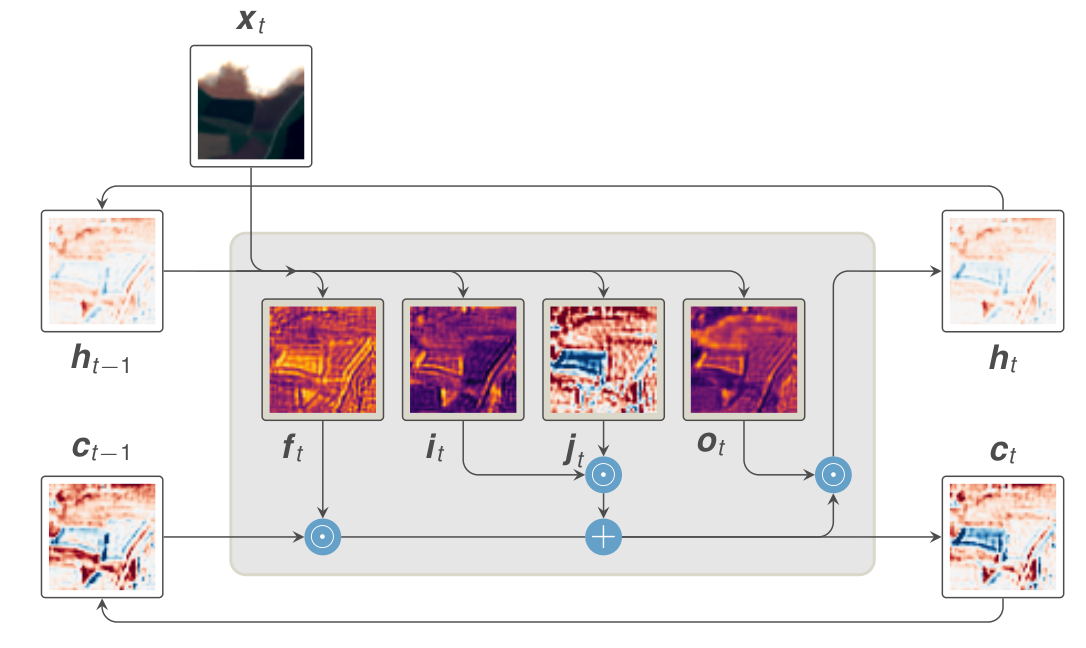
\includegraphics[width=\textwidth]{images/convlstm}	
		%\lstmexplain
	\end{column}
\end{columns}



\end{frame}

\begin{frame}
\frametitle{Classification ConvLSTM Network}

\centering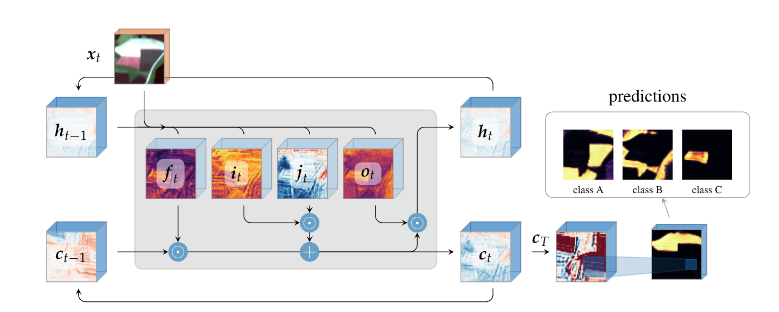
\includegraphics[width=.8\textwidth]{images/lstm}

	\small
\textsl{
	Rußwurm M., Körner M. (2018). \textbf{Multi-Temporal Land Cover Classification with Sequential Recurrent Encoders}. In ISPRS International Journal of Geo-Information. 
}

\end{frame}


%{
%	\setbeamercolor{background canvas}{bg=tumbluedark}

\begin{frame}

\vfill
\Huge\color{black}
\begin{center}
	\begin{columns}
		\column{\textwidth}
		
		
		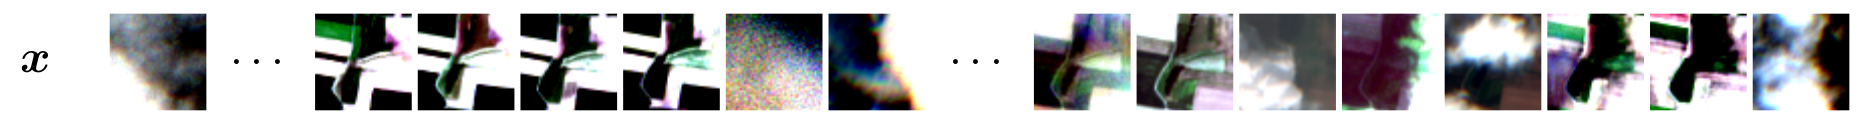
\includegraphics[width=\textwidth]{images/x_1}
		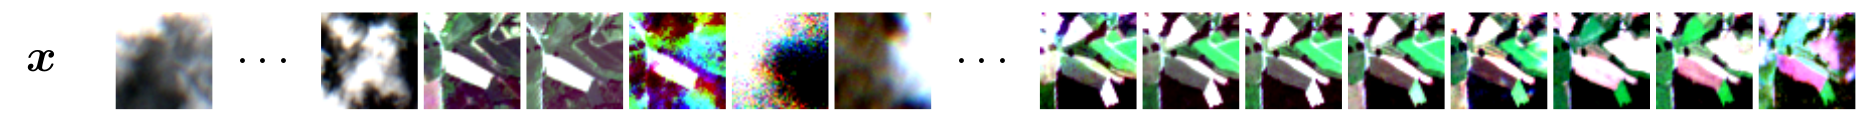
\includegraphics[width=\textwidth]{images/x_2}
		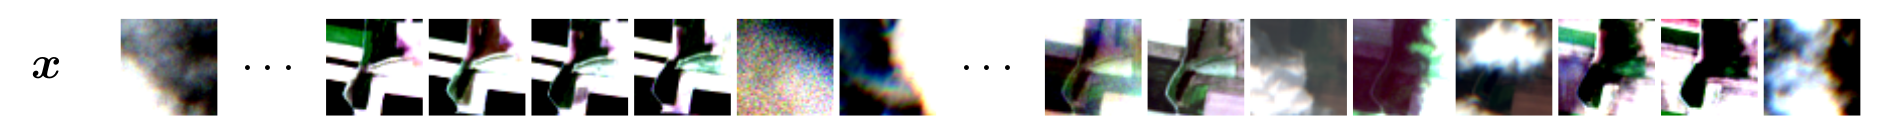
\includegraphics[width=\textwidth]{images/x_3}
		
		\vspace{3em}
		
		
		\textbf{\color{tumbluedark}Surprise:} 
		\hfill It worked without specifically labeling clouds!
%		\only<1>{Surprise:} \only<2>{It worked without labeling clouds!}
		%			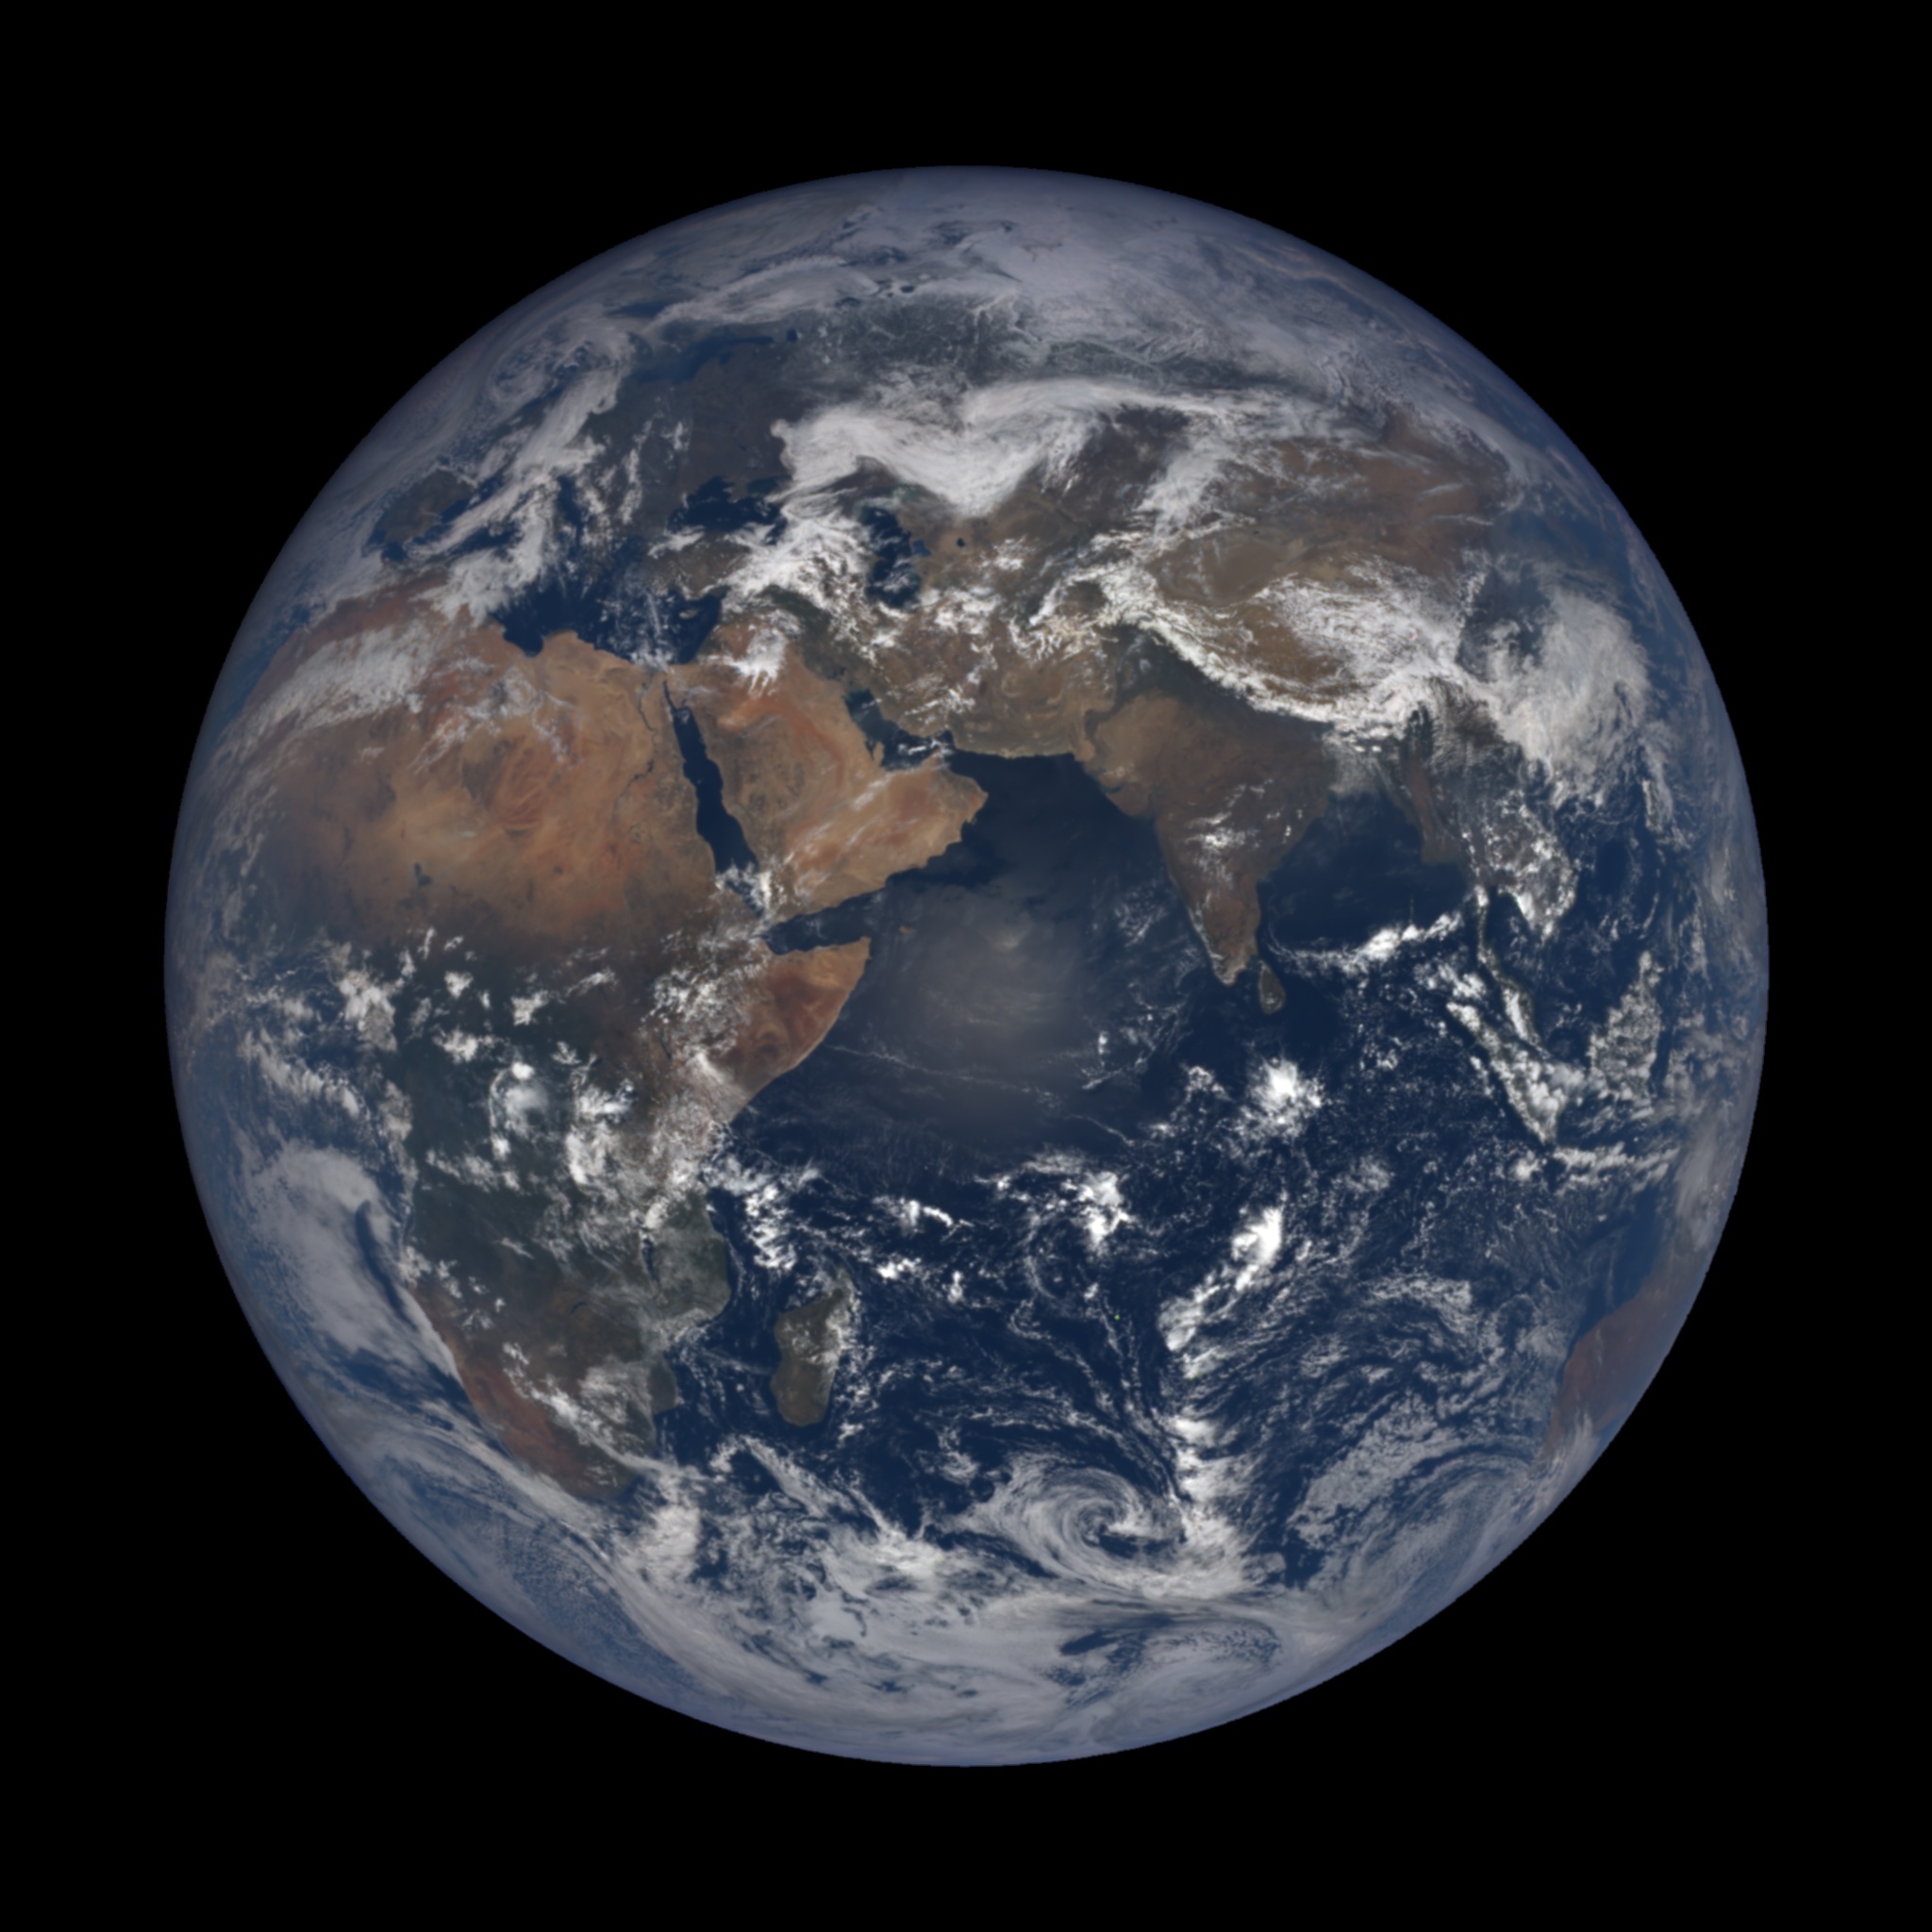
\includegraphics[width=5cm]{images/dscovrepic/epic1}
		%\includegraphics[width=7cm]{images/fdl}
	\end{columns}
\end{center}

\vfill

\end{frame}
%}

\begin{frame}
\frametitle{ConvLSTM robust to clouds}

\usepgfplotslibrary{groupplots}

\tikzsetnextfilename{scl}
\begin{tikzpicture}

%\def\data{images/classhist/classHistograms.dat}
\def\data{images/clouds/scl2.csv}

\pgfplotsset{ every non boxed x axis/.append style={x axis line style=-},
	every non boxed y axis/.append style={y axis line style=-}}

\pgfplotsset{every axis/.append style={ybar=1pt, bar width=6pt, ymajorgrids}}
\pgfplotsset{every axis label/.append style={font=\footnotesize},tick pos=left,ylabel near ticks}
\pgfplotsset{every tick label/.append style={font=\scriptsize}}
%\pgfplotsset{every x tick label/.append style={anchor=east,font=\tiny}}
%   \pgfplotsset{every y tick label/.append style={/pgf/number format/.cd, fixed, precision=2, fixed zerofill,}}
%\tikzstyle{caption}=[font=\footnotesize, fill=tumwhite, fill opacity=.5, text opacity=1]


\begin{axis}[
%group style={
%	%       group size=1 by 4,
%	group size=1 by 1,
%	xlabels at=edge bottom,
%	xticklabels at=edge bottom,
%	ylabels at=edge left,
%	yticklabels at=edge left,
%	vertical sep=2pt,
%	horizontal sep=2pt
%},
width=\textwidth,
height=3cm,
%ymode=log,
%log origin=infty,
%     y dir=reverse,
%     scaled ticks=true,
%log ticks with fixed point,
%scaled x ticks=true,
axis lines=left,
xlabel={image acquisition dates},
ylabel={cloud coverage},
xlabel style={yshift=-2mm},
xmin=-.5,
xmax=46,
%xlabel=clouds,
ytick={1,10,25,50,100},
yticklabels={\SI{1}{\percent},\SI{10}{\percent},\SI{25}{\percent},\SI{50}{\percent},\SI{100}{\percent}},
xtick=data,
xticklabels={
%	03. Jan,
%	13. Jan,
%	20. Jan,
%	21. Jan,
%	28. Jan,
%	12. Feb,
%	11. Mär,
%	20. Mär,
%	23. Mär,
%	03. Apr,
%	13 Apr.,
%	19. Apr,
%	22. Apr,
%	29. Apr,
%	02. Mai,
%	10. Mai,
%	22. Mai,
%	29. Mai,
%	08. Jun,
%	18. Jun,
%	28. Jan,
%	02. Jul,
%	14. Jul,
%	18. Jul,
%	21. Jul,
%	28. Jul,
%	30. Jul,
%	07. Aug,
%	17. Aug,
%	20. Aug,
%	28. Aug,
%	21. Aug,
%	09. Sep.,
%	12. Sep..,
%	18. Sep.,
%	26. Sep.,
%	29. Sep.,
%	09. Okt.,
%	18. Okt.,
%	28. Okt.,
%	09. Nov.,
%	15. Nov.,
%	18. Nov.,
%	28. Nov.,
%	06. Dez.,
%	08. Dez.
},
axis on top
];

\addplot[
%       draw=tumblue,
draw=none,
fill=tumblue,rounded corners=.5pt
] table [col sep=comma, x=id, y=cloudpercent] {\data};


\end{axis}
\end{tikzpicture}
%usepgfplotslibrary{fillbetween}

%\newcommand{\fbopacity}{0.3}
%\newcommand{\skippoints}{2}


%\def\measure{oa}
\def\height{3.5cm}


%\colorlet{L1Ccolor}{tumblue}
%colorlet{L2Acolor}{tumblack}

%\colorlet{clouds01color}{tumred}
%\colorlet{clouds10color}{tumorange}
%\colorlet{clouds25color}{tumgray}
%\colorlet{clouds50color}{tumblue}
%\colorlet{clouds80color}{tumblack}

\colorlet{clouds01color}{tumbluedark!55}
\colorlet{clouds10color}{tumbluedark!70}
\colorlet{clouds25color}{tumbluedark!85}
\colorlet{clouds50color}{tumbluedark}
\colorlet{clouds80color}{tumblack}

\colorlet{highlightcolor}{tumgraylight!25}

%\colorlet{2017traincolor}{tumgray}
%\colorlet{2017testcolor}{tumblack}

\tikzset{new spy style/.style={spy scope={%
			magnification=2,
			connect spies,
			every spy on node/.style={
				rectangle,
				rounded corners=1pt,
				draw,
			},
			every spy in node/.style={
				draw,
				rectangle,
				rounded corners=1pt,
				fill=gray!40,
			}
		}
	}
} 


\tikzsetnextfilename{clouds}
\begin{tikzpicture}[new spy style, remember picture]
	
	% replaced by global settings in figures.tex
%	\pgfplotsset{every axis plot/.append style={line width=1pt}}
	
	
	\begin{groupplot}[
	group style={
		group size=2 by 1,
		xlabels at=edge bottom,
		ylabels at=edge left,
		xticklabels at=edge bottom,
		vertical sep=35pt,
		group name=trainplot
	},
	legend style={
		at={(1.65,0)},
		anchor=south,
		fill=tumgraylight!50,
		rounded corners=1pt,
		draw=none,
		font=\scriptsize, 
		legend image post style={line width =3pt},
		/tikz/every even column/.append style={column sep=0.2cm},
	},
	axis lines=left,
	grid=both,
	scaled x ticks = false,
	y tick label style={/pgf/number format/fixed},
	grid style={draw=tumgraylight},
	legend columns=1,
	width=.38\textwidth,
	height=\height,
	xlabel={samples seen},
	xmin=-10000,
	xmax=800000,
	ymin=.85,
	ymax=.95]


\nextgroupplot[title=,ylabel={ov. acc.},ymin=.2,ymax=1]


\coordinate (topsource) at (axis cs: 800000,.96);
\coordinate (bottomsource) at (axis cs: 800000,.84);

\coordinate (topsourceleft) at (axis cs: 0,.96);
\coordinate (bottomsourceleft) at (axis cs: 0,.84);

\fill[highlightcolor,draw=tumgraylight, rounded corners=1pt] (bottomsource) -- (bottomsourceleft) -- (topsourceleft) -- (topsource); 

\addplot[clouds01color, forget plot] table [x=Step, y = clouds01_test2016clouds01_oa, col sep=comma] {images/clouds/train_rw3.csv};

\addplot[clouds10color, forget plot] table [x=Step, y = clouds10_test2016clouds10_oa, col sep=comma] {images/clouds/train_rw3.csv};

\addplot[clouds25color, forget plot] table [x=Step, y = clouds25_test2016clouds25_oa, col sep=comma] {images/clouds/train_rw3.csv};

\addplot[clouds50color, forget plot] table [x=Step, y = clouds50_test2016clouds50_oa, col sep=comma] {images/clouds/train_rw3.csv};

\addplot[clouds80color, forget plot] table [x=Step, y = clouds80_test2016_oa, col sep=comma] {images/clouds/train_rw3.csv};

\nextgroupplot[
	title=,
	ylabel={ov. acc.}, 
	ymin=.84,
	ymax=.96, 
	xmin=0,
	axis y line*=right,
	ylabel near ticks, 
	yticklabel pos=right,
	grid=both,
	grid style={tumgray!50},
	axis background/.style={fill=highlightcolor},
	]
\addplot[clouds01color] table [x=Step, y = clouds01_test2016clouds01_oa, col sep=comma] {images/clouds/train_rw15.csv};
\addlegendentry{$<$ \SI{1}{\percent} (4 obs.)}

\addplot[clouds10color] table [x=Step, y = clouds10_test2016clouds10_oa, col sep=comma] {images/clouds/train_rw15.csv};
\addlegendentry{$<$ \SI{10}{\percent} (10 obs.)}

\addplot[clouds25color] table [x=Step, y = clouds25_test2016clouds25_oa, col sep=comma] {images/clouds/train_rw15.csv};
\addlegendentry{$<$ \SI{25}{\percent} (17 obs.)}

\addplot[clouds50color] table [x=Step, y = clouds50_test2016clouds50_oa, col sep=comma] {images/clouds/train_rw15.csv};
\addlegendentry{$<$ \SI{50}{\percent} (23 obs.)}

\addplot[clouds80color] table [x=Step, y = clouds80_test2016_oa, col sep=comma] {images/clouds/train_rw15.csv};
\addlegendentry{all images (46 obs.)}

\coordinate (toptarget) at (rel axis cs: 0,1);
\coordinate (bottomtarget) at (rel axis cs: 0,0);

\end{groupplot}

\draw[fill=highlightcolor, draw=tumgraylight] (topsource) -- (toptarget) -- (bottomtarget)  -- (bottomsource);
\draw[|-|, tumgray] ($ (bottomsource) + (0ex,0) $) -- ($ (topsource) + (0ex,0) $);
\draw[|-|, tumgray] (bottomtarget) -- (toptarget);

\end{tikzpicture}  

\end{frame}


\begin{frame}
	\frametitle{Remembering Karpathy's "Unreasonable Effectiveness of RNNs"}
	
	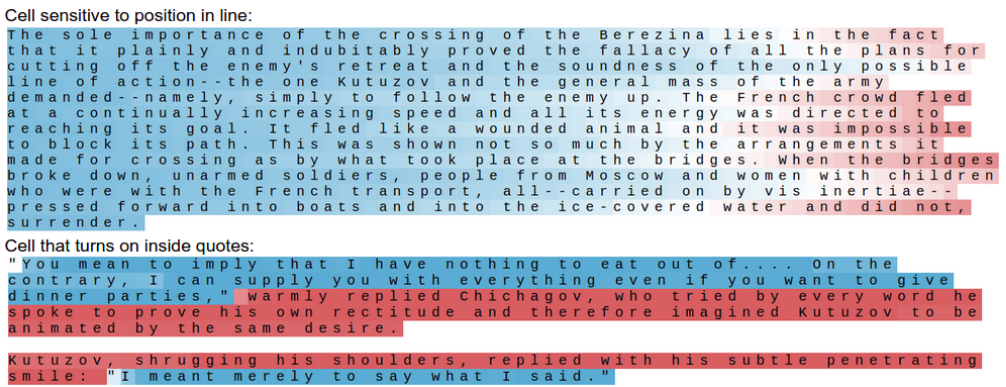
\includegraphics[width=\textwidth]{images/karpathy}
	
	\url{http://karpathy.github.io/2015/05/21/rnn-effectiveness/}
\end{frame}

\newcounter{tcounter}

\newcommand{\drawcbar}[5]{
	\def\tnode{#1} % iGate0
	\def\cmap{#2} % inferno
	\def\cbarheight{#3} % 1cm
	%	\def\vmin{#4} % 0
	%	\def\vmax{#5} % 1
	
	\node[xshift=1mm] (cbar\tnode) at (\tnode.east){\includegraphics[height=2mm, width=\cbarheight, angle=90,origin=c]{\cmap}};
	\node[anchor=south] at (cbar\tnode.south east) {\tiny #4};
	\node[anchor=north] at (cbar\tnode.north east) {\tiny #5};
}
\newcommand{\imagecolumns}[2]{
		\foreach \t in {#1,...,#2}{
			\node(times) at (\thetcounter*\hdist,0*\vdist){$t_{\the\numexpr\t+1\relax}$};
			\node[activation](xlast) at (\thetcounter*\hdist,-1*\vdist){\includegraphics[width=\imagewidth]{\folder/sample\s/time\t_x}};
			
			\node[activation, yshift=-1mm](flast1) at (\thetcounter*\hdist,-2*\vdist){\includegraphics[width=\imagewidth]{\folder/sample\s/time\t/\done_fGate}};
			\node[activation, yshift=-1mm](ilast1) at (\thetcounter*\hdist,-3*\vdist){\includegraphics[width=\imagewidth]{\folder/sample\s/time\t/\done_iGate}};
			\node[activation, yshift=-1mm](jlast1) at (\thetcounter*\hdist,-4*\vdist){\includegraphics[width=\imagewidth]{\folder/sample\s/time\t/\done_jGate}};
			\node[activation, yshift=-1mm](clast1) at (\thetcounter*\hdist,-5*\vdist){\includegraphics[width=\imagewidth]{\folder/sample\s/time\t/\done_state}};
			
			\stepcounter{tcounter}
		}
	}
	
\newcommand{\dotscolumn}{
	\node[activation] at (\thetcounter*\hdist,-1*\vdist){$\dots$};
	
	\node[activation,yshift=-1mm] at (\thetcounter*\hdist,-2*\vdist){$\dots$};
	\node[activation,yshift=-1mm] at (\thetcounter*\hdist,-3*\vdist){$\dots$};
	\node[activation,yshift=-1mm] at (\thetcounter*\hdist,-4*\vdist){$\dots$};
	\node[activation,yshift=-1mm] at (\thetcounter*\hdist,-5*\vdist){$\dots$};
	\stepcounter{tcounter}
	}

\newcommand{\figactivations}[2]{
	% 1: number of sample
	% 2. number of activation
	
	\setcounter{tcounter}{0}
	
	\begin{tikzpicture}
	%\figGates{0}{18}{1}{3}
	\def\folder{images/activations/48px}
	
	\tikzstyle{activation}=[]
	\def\s{#1}
	
	\def\done{#2}
%	\def\dtwo{22}
%	\def\dthree{47}
	
	%% grid distance vertical and horizontal
	\def\vdist{8.5mm}
	\def\hdist{8.5mm}
	
	\def\imagewidth{8mm}
	
	
	%% descriptions top row
	\node[anchor=west] at (-1.5*\hdist,-1*\vdist){$\V{x}$};
	\node[anchor=west, yshift=-1mm](f1) at (-1.5*\hdist,-2*\vdist){$\V{f}^{(\done)}$};
	\node[anchor=west, yshift=-1mm](i1) at (-1.5*\hdist,-3*\vdist){$\V{i}^{(\done)}$};
	\node[anchor=west, yshift=-1mm](j1) at (-1.5*\hdist,-4*\vdist){$\V{j}^{(\done)}$};
	\node[anchor=west, yshift=-1mm](c1) at (-1.5*\hdist,-5*\vdist){$\V{c}^{(\done)}$};


	\imagecolumns{0}{1}
	\dotscolumn
	\imagecolumns{9}{14}
	\dotscolumn
	\imagecolumns{30}{34}
	
	
	\drawcbar{flast1}{images/activations/inferno}{\imagewidth}{0}{1}
	\drawcbar{ilast1}{images/activations/inferno}{\imagewidth}{0}{1}
	\drawcbar{jlast1}{images/activations/RdBu_r}{\imagewidth}{-1}{1}
	\drawcbar{clast1}{images/activations/RdBu_r}{\imagewidth}{-1}{1}
	
	
	
	\end{tikzpicture}
}
\begin{frame}
\frametitle{Internal States Encode increasingly Classification Features}
\framesubtitle{LSTM cell \textbf{47} of 256}
\figactivations{1}{3}
\end{frame}
%

\begin{frame}
\frametitle{Found Cloud Masking Cells in the RNN}
\framesubtitle{LSTM cell \textbf{47} of 256}
\figactivations{1}{22}
\end{frame}

\begin{frame}
\frametitle{Found Cloud Masking Cells in the RNN}
\framesubtitle{LSTM cell \textbf{47} of 256}
\figactivations{1}{47}
\end{frame}
%
%\begin{frame}
%	\frametitle{Publication and Github}
%	
%			Including the spatial information by adding convolutions
%	\vspace{2em}
%	{\small
%		Rußwurm, M., \& Körner, M. (2018). Multi-temporal land cover classification with sequential recurrent encoders. ISPRS International Journal of Geo-Information, 7(4), 129.
%	}
%
%	Github
%	\url{https://github.com/tum-lmf/mtlcc}
%	
%\end{frame}


\begin{frame}[c]
\frametitle{Paper and Code}
\centering 

%	\vspace{3em}

\large



Github + DockerHub + Continuation with GAF AG

\vspace{1ex}


\includegraphics[width=2cm]{images/github} \hspace{.5ex}

\includegraphics[width=2cm]{images/qr_github} \hspace{.5ex}

\includegraphics[width=2cm]{images/docker} \hspace{.5ex}
\vline
\hspace{.5ex}

\includegraphics[width=4cm]{images/gaf}

\vspace{1ex}

\url{https://github.com/TUM-LMF/MTLCC}
\url{https://github.com/TUM-LMF/MTLCC-pytorch}

\url{http://www.lmf.bgu.tum.de/vision/}

\vspace{1em}
\begin{columns}[t]
	\column{.5\textwidth}
	\scriptsize
	\textsl{
		Rußwurm, M. and Körner, M. (2017). \textbf{Temporal Vegetation Modelling using Long Short-Term Memory Networks for Crop Identification from Medium-Resolution Multi-Spectral Satellite Images}. In IEEE/ISPRS EarthVision 2017 Workshop, Proceedings of the IEEE CVPR Workshops.
	}
	
	\column{.5\textwidth}
	\small
	\textsl{
		Rußwurm M., Körner M. (2018). \textbf{Multi-Temporal Land Cover Classification with Sequential Recurrent Encoders}. ISPRS International Journal of Geo-Information. https://arxiv.org/abs/1802.02080. (in review)
	}
	
\end{columns}


\end{frame}

%\begin{frame}
%\frametitle{Found Cloud Masking Cells in the RNN}
%\framesubtitle{LSTM cell \textbf{47} of 256}
%\figactivations{1}{3}
%\end{frame}
